%===============================================================================
% LaTeX sjabloon voor de bachelorproef toegepaste informatica aan HOGENT
% Meer info op https://github.com/HoGentTIN/bachproef-latex-sjabloon
%===============================================================================

\documentclass{bachproef-tin}

\usepackage{hogent-thesis-titlepage} % Titelpagina conform aan HOGENT huisstijl
\usepackage[utf8]{inputenc}
\usepackage[english]{babel}
\usepackage{listings}
\usepackage{graphics}
\usepackage{graphicx}
\usepackage[backend=biber]{biblatex}
\usepackage{caption}
\usepackage{hyperref}

\usepackage{kantlipsum}
\usepackage{xcolor}
\usepackage{import}
\definecolor{LightGray}{gray}{0.9}
%\definecolor{DarkGray}{gray}{0.1}

%\pagecolor{DarkGray}


%New colors defined below
\definecolor{codegreen}{rgb}{0,0.6,0}
\definecolor{codegray}{rgb}{0.5,0.5,0.5}
\definecolor{codepurple}{rgb}{0.58,0,0.82}
\definecolor{backcolour}{rgb}{0.95,0.95,0.92}
%%---------- Documenteigenschappen ---------------------------------------------
% TODO: Vul dit aan met je eigen info:
  
% De titel van het rapport/bachelorproef
\title{Handschriftherkenning voor doktersbriefjes m.b.v. Azure Computer Vision}

% Je eigen naam
\author{Helmi Dayyeh}

% De naam van je promotor (lector van de opleiding)
\promotor{Irina Malfait} % controlleren of beide namen volledig juist zijn !

% De naam van je co-promotor. Als je promotor ook je opdrachtgever is en je
% dus ook inhoudelijk begeleidt (en enkel dan!), mag je dit leeg laten.
\copromotor{Wouter Baetens}

% Indien je bachelorproef in opdracht van/in samenwerking met een bedrijf of
% externe organisatie geschreven is, geef je hier de naam. Zoniet laat je dit
% zoals het is.
\instelling{Arinti} % ?

% Academiejaar
\academiejaar{2019-2020}

% Examenperiode
%  - 1e semester = 1e examenperiode => 1
%  - 2e semester = 2e examenperiode => 2
%  - tweede zit  = 3e examenperiode => 3
\examenperiode{2}

%===============================================================================
% Inhoud document
%===============================================================================

\begin{document}

%---------- Taalselectie -------------------------------------------------------
% Als je je bachelorproef in het Engels schrijft, haal dan onderstaande regel
% uit commentaar. Let op: de tekst op de voorkaft blijft in het Nederlands, en
% dat is ook de bedoeling!

%\selectlanguage{english}

%---------- Titelblad ----------------------------------------------------------
\inserttitlepage
%---------- Samenvatting, voorwoord --------------------------------------------
\usechapterimagefalse
%%=============================================================================
%% Voorwoord
%%=============================================================================

\chapter*{\IfLanguageName{dutch}{Woord vooraf}{Preface}}
\label{ch:voorwoord}

%% TODO:
%% Het voorwoord is het enige deel van de bachelorproef waar je vanuit je
%% eigen standpunt (``ik-vorm'') mag schrijven. Je kan hier bv. motiveren
%% waarom jij het onderwerp wil bespreken.
%% Vergeet ook niet te bedanken wie je geholpen/gesteund/... heeft
Deze bachelorscriptie werd geschreven met het oog op het behalen van de titel: Bachelor in de Toegepaste Informatica. 


Naar aanleiding van mijn stage bij De Cronos Groep, leek het de perfecte opportuniteit om in het domein van Cloud Computing en Artificiële intelligentie een onderzoek te starten. Hierbij kwam Arinti (een dochterbedrijf van De Cronos Groep) met een zeer interessant onderzoeksvoorstel.  De Christelijke Mutualiteit had namelijk problemen met het lezen van doktersgeschrift op medische voorschriften. Hierbij kwam de vraag of dit proces eveneens geautomatiseerd kon worden door gebruik te maken van AI, en of er een verschil zou zijn in performantie/accuraatheid.  


Aangezien het voorstel van dit onderzoek mij aangeboden werd vanuit Arinti, wil ik mijn co-promoter, Wouter Baetens bedanken om mij de kans te geven om dit zeer interessant onderzoek uit te voeren en enige vragen te beantwoorden die naar boven kwamen. Ook wil ik mijn stagebegeleider, Geert Baeke, bedanken om mij voor te stellen aan Arinti en zo aanleiding tot dit onderzoek te geven. Verder bedank ik mijn promotor, Irina Malfait, voor de snelle feedback en sturing van de bachelorproef. 

Tot slot wil ik mijn ouders en vrienden bedanken voor de constante steun bij het uitvoeren van dit onderzoek. 
%%=============================================================================
%% Samenvatting
%%=============================================================================

% TODO: De "abstract" of samenvatting is een kernachtige (~ 1 blz. voor een
% thesis) synthese van het document.
%
% Deze aspecten moeten zeker aan bod komen:
% - Context: waarom is dit werk belangrijk?
% - Nood: waarom moest dit onderzocht worden?
% - Taak: wat heb je precies gedaan?
% - Object: wat staat in dit document geschreven?
% - Resultaat: wat was het resultaat?
% - Conclusie: wat is/zijn de belangrijkste conclusie(s)?
% - Perspectief: blijven er nog vragen open die in de toekomst nog kunnen
%    onderzocht worden? Wat is een mogelijk vervolg voor jouw onderzoek?
%
% LET OP! Een samenvatting is GEEN voorwoord!

%%---------- Nederlandse samenvatting -----------------------------------------
%
% TODO: Als je je bachelorproef in het Engels schrijft, moet je eerst een
% Nederlandse samenvatting invoegen. Haal daarvoor onderstaande code uit
% commentaar.
% Wie zijn bachelorproef in het Nederlands schrijft, kan dit negeren, de inhoud
% wordt niet in het document ingevoegd.

\IfLanguageName{english}{%
\selectlanguage{dutch}
\chapter*{Samenvatting}
\lipsum[1-4]
\selectlanguage{english}
}{}

%%---------- Samenvatting -----------------------------------------------------
% De samenvatting in de hoofdtaal van het document

\chapter*{\IfLanguageName{dutch}{Samenvatting}{Abstract}}

In dit onderzoek werd er gekeken naar de limitaties van handschriftherkenning. Hierbij werd de vraag gesteld of door wijze van handschriftherkenning de Christelijke Mutualiteit een meerwaarde zou zien bij het lezen van doktersvoorschriften. Met de evoluerende opkomst van Artificiële intelligentie, zijn zaken waar vroeger fysieke werkkrachten voor ingezet werden, in een handgreep geautomatiseerd. Hierdoor wordt de nood aan extra kosten binnen een bedrijf geëlimineerd. Bovendien zijn mensen gekend om fouten te maken en kan dit een negatieve invloed op de workflow binnen het bedrijf veroorzaken. 



De eerste taak bij dit onderzoek was de nood aan een literatuurstudie. Hierbij werd tot in detail beschreven wat de evolutie in het domein van handschriftherkenning doorheen de jaren ondergaan heeft en waar onderzoek in dit domein hedendaags toe gekomen is. 



De literatuurstudie bracht ons tot enkele cruciale ondervindingen. Om mogelijks een conclusie te trekken uit deze onderzoeksvraag, zou in de eerste plaats een Machine Learning model nodig zijn, dat getraind is op de voorspelling van medische terminologie. Na enig opzoekwerk, bleek dat het verzamelen van de data nodig voor dit model, een probleem zou vormen. Doktersvoorschriften worden als een confidentiële vorm van data beschouwd binnen dit domein en worden niet zomaar vrijgegeven. Een op maat gemaakt model bleek dus geen mogelijkheid te zijn voor dit onderzoek.  



Hierbij kwam het idee om gebruik te maken van Cloud Computing, men zou dan gebruik maken van een voorgetraind model dat aangeboden werd door een derde partij. Naar aanleiding van de stage, werd gekozen om gebruik te maken van de oplossingen die Microsoft te bieden heeft. Meer bepaald de Azure Computer Vision service. Met een instantie van deze service kan men eenvoudige API requests versturen die vervolgens een doeltreffend resultaat leverden door de Cloud in de achtergrond het werk te laten uitvoeren.  



Om dit tenslotte op de proef te stellen, werden enkele test cases opgezet, waarbij verscheidene obstakels die zouden kunnen voorkomen, getest werden. Enerzijds werd hiervoor gebruik gemaakt van een test groep. Aan deze testgroep werden enkele doktersvoorschriften voorgesteld en werd gevraagd deze zo accuraat mogelijk te interpreteren. Vervolgens werd deze interpretatie vergeleken met de resulterende data van de API. Men kon hierdoor nagaan of artificiële intelligentie bepaalde woorden beter zou kunnen voorspellen dan mensen. 



De accuraatheid hiervan werd deels ook op de proef gesteld door testen uit te voeren met een verlaagde resolutie en variërende positionering van personengegevens. Uit deze testen kon men concluderen dat doktersgeschrift wel degelijk met een relatief hoge accuraatheid en snelheid geëxtraheerd kon worden van voorschriften.  



Dit proces zou op eenvoudige wijze in een productieomgeving ingezet kunnen worden, waardoor de Christelijke Mutualiteit een meerwaarde zou zien in processnelheid en accuraatheid. Aangezien dit onderzoek gebruik maakte van Engelse voorschriften, zou met verder onderzoek naar de extractie van Nederlandse voorschriften, een volledigere conclusie getrokken kunnen worden. 


%---------- Inhoudstafel -------------------------------------------------------
\pagestyle{empty} % Geen hoofding
\tableofcontents  % Voeg de inhoudstafel toe
\cleardoublepage  % Zorg dat volgende hoofstuk op een oneven pagina begint
\pagestyle{fancy} % Zet hoofding opnieuw aan

%---------- Lijst figuren, afkortingen, ... ------------------------------------

% Indien gewenst kan je hier een lijst van figuren/tabellen opgeven. Geef in
% dat geval je figuren/tabellen altijd een korte beschrijving:
%
%  \caption[korte beschrijving]{uitgebreide beschrijving}
%
% De korte beschrijving wordt gebruikt voor deze lijst, de uitgebreide staat bij
% de figuur of tabel zelf.

\listoffigures
\listoftables

% Als je een lijst van afkortingen of termen wil toevoegen, dan hoort die
% hier thuis. Gebruik bijvoorbeeld de ``glossaries'' package.
% https://www.overleaf.com/learn/latex/Glossaries

%---------- Kern ---------------------------------------------------------------

% De eerste hoofdstukken van een bachelorproef zijn meestal een inleiding op
% het onderwerp, literatuurstudie en verantwoording methodologie.
% Aarzel niet om een meer beschrijvende titel aan deze hoofstukken te geven of
% om bijvoorbeeld de inleiding en/of stand van zaken over meerdere hoofdstukken
% te verspreiden!

%%=============================================================================
%% Inleiding
%%=============================================================================

\chapter{\IfLanguageName{dutch}{Inleiding}{Introduction}}
\label{ch:inleiding}

Integratie van artificiële intelligentie in alledaagse workflows is een trend die meer en meer uitgeoefend wordt. Met de opkomst van artificiële intelligentie kan men eenvoudige taken die fysieke werkkrachten vereisen automatiseren. Hierdoor besparen bedrijven de tijd en het budget dat kruipt in het aanwerven en uitbetalen van personeel. Bovendien ligt het aantal transacties dat dergelijke software kan verwerken veel hoger dan hetgeen dat menselijke intuïtie kan bereiken. De taken die hierbij geautomatiseerd kunnen variëren van spraakherkenning systemen met realtime transcriptie tot handschriftherkenning op postbrieven om zo het juiste adres te achterhalen. Het herkennen van handgeschreven karakters was één van de eerste toepassingen die met de opkomst van AI verwezenlijkt kon worden. Toepassingen zoals deze kunnen vandaag de dag al volledige handgeschreven documenten omzetten naar machinale tekst met behulp van een gepast machine learning framework.  

Hieruit komt de Christelijke Mutualiteit met de vraag of men deze technologie kan gebruiken om het typische doktersgeschrift dat men terugvindt op voorschriften te achterhalen. Het is een typische gezegde dat het handgeschrift van dokters praktisch onleesbaar is en dit blijkt zo uit de vraag naar een oplossing hiervoor. 

Er zijn verscheidene spelers op de markt wanneer het komt om een performant AI-systeem op te bouwen. Grote spelers zoals Microsoft en Google hebben hun eigen cloud architecturen die gebruik maken van de enorme hoeveelheid data die zij verzameld hebben door de jaren heen. Aangezien de accuraatheid van een AI-systeem gepaard gaat met de hoeveelheid data die gebruikt wordt voor training spreekt het van zichzelf dat Microsoft en Google marktleiders zijn in dit veld. Er zijn echter naast deze twee oplossingen ook nog open source toepassingen die niet onderschat mogen worden.  


\section{\IfLanguageName{dutch}{Probleemstelling}{Problem Statement}}
\label{sec:probleemstelling}

In sommige gevallen kan het voorvallen dat wanneer men een voorschrift ingeeft bij de Christelijke Mutualiteit, het handgeschrift op dit voorschrift onleesbaar is. Dit vormt een probleem wanneer men medische kosten terug wil betalen. Het is duidelijk dat de tijd die de mensen gebruiken om dit handgeschrift te ontcijferen verloren gaat. Daarom zou een geautomatiseerd systeem dit probleem kunnen verminderen. Aangezien dit veld nog redelijk recent is, is het niet onrealistisch dat een foute voorspelling kan gebeuren. De meerderheid van deze systemen maken gebruik van recurrent neuraal netwerk, wat betekent dat het systeem foute voorspellingen onthoudt en zichzelf aanpast naargelang specifieke kenmerken terugkeren. Hierdoor kan het systeem zich specialiseren in een domein waar bv. veel medische termen terugkomen. 

\section{\IfLanguageName{dutch}{Onderzoeksvraag}{Research question}}
\label{sec:onderzoeksvraag}


De vraag waarop de uitkomst van dit onderzoek uiteindelijk zal op antwoorden is of het wel degelijk mogelijk is om dokters handgeschrift te extraheren van doktersbriefjes. In welke zin varieert dokters handgeschrift van een ander en heeft dit invloed op de herkenning?  De focus hierbij ligt op de efficiëntie van de gebruikte oplossing, in het geval van dit onderzoek zal de herkenningsfase in het praktische gedeelte gebruik maken van Azure Computer Vision. Dit omvat grotendeels de hoofdonderzoeksvraag, echter kan deze vraag nog opgedeeld worden in verschillende deelvragen. 
\begin{itemize}
  \item  Welke factoren bepalen de accuraatheid? 
  \item  Worden medische termen even accuraat vertaald als normale tekst? 
  \item  Kan men deze oplossing hergebruiken voor andere doeleinden? 
  \item  In hoeverre maakt zelf ingebrachte data een verschil op het resultaat? 
\end{itemize}

\section{\IfLanguageName{dutch}{Onderzoeksdoelstelling}{Research objective}}
\label{sec:onderzoeksdoelstelling}

De uiteindelijke conclusie van dit onderzoek zal aantonen dat dergelijke software ontwikkelt kan worden om het probleem dat doktersgeschrift met zich meebrengt op te lossen. Wanneer de software levert wat er gevraagd wordt kan dit onderzoek als succesvol verklaard worden. Een accuraatheid van +- 74 \% zou aantonen dat het systeem met een degelijke accuraatheid de extractie kan uitvoeren. In het domein van handschrift extractie wordt dit gezien als een hoog percentage. Percentages bij geprinte tekst liggen veel hoger aangezien een font eenzelfde lettertype/lettergrootte aanhoudt. Uiteraard is het ook van belang dat de CM een meerwaarde ziet in het gebruik van deze software. Hierbij zal men rechtstreeks doktersbriefjes kunnen inscannen en meteen ook een digitale versie verkrijgen van de inhoud.  

\section{\IfLanguageName{dutch}{Opzet van deze bachelorproef}{Structure of this bachelor thesis}}
\label{sec:opzet-bachelorproef}

% Het is gebruikelijk aan het einde van de inleiding een overzicht te
% geven van de opbouw van de rest van de tekst. Deze sectie bevat al een aanzet
% die je kan aanvullen/aanpassen in functie van je eigen tekst.

De rest van deze bachelorproef is als volgt opgebouwd:

In Hoofdstuk~\ref{ch:stand-van-zaken} wordt een overzicht gegeven van de stand van zaken binnen het onderzoeksdomein, op basis van een literatuurstudie.

In Hoofdstuk~\ref{ch:methodologie} wordt de methodologie toegelicht en worden de gebruikte onderzoekstechnieken besproken om een antwoord te kunnen formuleren op de onderzoeksvragen.

% TODO: Vul hier aan voor je eigen hoofstukken, één of twee zinnen per hoofdstuk

In Hoofdstuk~\ref{ch:conclusie}, tenslotte, wordt de conclusie gegeven en een antwoord geformuleerd op de onderzoeksvragen. Daarbij wordt ook een aanzet gegeven voor toekomstig onderzoek binnen dit domein.
\chapter{\IfLanguageName{dutch}{Stand van zaken}{State of the art}}
\label{ch:stand-van-zaken}

% Tip: Begin elk hoofdstuk met een paragraaf inleiding die beschrijft hoe
% dit hoofdstuk past binnen het geheel van de bachelorproef. Geef in het
% bijzonder aan wat de link is met het vorige en volgende hoofdstuk.

% Pas na deze inleidende paragraaf komt de eerste sectiehoofding.

Handschriftherkenning, het woord zegt het zelf al. Het digitalseren van handgeschreven tekst is een veelgebruikte technologie die al sinds de jaren 60 in de maak is en dagelijks talloze transacties automatiseert. Een handgeschreven adres op een brief digitaliseren of fysieke documenten converteren naar een pdf formaat elimineren de nood aan fysieke werkkrachten in verscheidene sectoren en verhogen de efficiëntie. De manier waarop een computertekst transformeert naar zijn digitale tegenligger is niet zo voor de hand liggend en gebruikt in de meeste gevallen een combinatie van technieken die over de jaren heen ontwikkeld werden.
\newline
\newline
Aangezien dit onderzoek de focus legt op tekst extractie, zullen de verscheidene technologieën die handschriftherkenning mogelijk maakt, besproken worden om zo een duidelijk overzicht te geven over wat er precies gebeurt. 
Na deze korte introductie zal het Azure computer Vision framework van Microsoft aangereikt worden. Dit is één van de meer modernere oplossingen die centraal staan bij het praktische gedeelte van dit onderzoek en die het herkennen van handgeschreven teksten vergemakkelijkt.
\section{Optical Character Recognition}
 
OCR (Optical Character Recognition) analyseert de vorm en de complexiteit van een bitsgewijs gemapt karakter en geeft deze vervolgens een waarde. Tegenwoordig kan de meeste OCR software zeer accurate resultaten weergeven als het op machinaal afgedrukte teksten neerkomt. Dit is zeker van toepassing wanneer er een duidelijke font met eenzelfde lengte tussen de karakters gebruikt wordt. \newline \newline Wat echter een groter probleem is dat zich kan voordoen is variabele lengte van karakters, onbekende fonts en al zeker handgeschreven teksten. (\cite{Breithaupt2014}) 



OCR wordt vandaag de dag in een enorm aantal toepassingen gebruikt, zoals het transcriberen van brieven en in zelfrijdende auto's door het herkennen van snelheidslimieten op borden. 

De technologische vordering in dit domein groeit dagelijks en zal in de toekomst enkel maar verbeteren. Echter, de accuraatheid van OCR is verre van perfect en vergt nog altijd een of andere vorm van menselijk toezicht. Op een pagina die 30 karakters telt zal zelfs een dergelijke OCR toepassing met 99 \% accuraatheid, een gemiddelde van 30 fouten maken. Aangezien dit percentage van toepassing is op machinaal geschreven tekst, zal een OCR toepassing losgelaten op handgeschreven tekst een drastisch lager accuraatheidspercentage kennen. (\cite{Nagy1999}) 
\newline \newline
Technieken gebruikt bij het herkennen van handgeschreven woorden maken doorgaans gebruik van holistische of analytische strategieën voor de training en recognition fase. Holistische strategieën maken doorgaans gebruik van een top-down approach voor het herkennen van het volledige woord, hierdoor elimineert men problemen die zich voordoen bij de segmentatie fase. Bij deze strategie worden globale kenmerken van het volledige woord geëxtraheerd en worden vervolgens gebruikt bij herkenning van woorden in een kleine lexicografische omgeving. Analytische strategieën maken gebruik van een bottom-up approach. Expliciete segmentatie van woorden in karakters is nodig voor deze aanpak aangezien deze strategie geïsoleerde karakters herkent. Hierdoor is men niet gelimiteerd door een specifieke lexicografische omgeving maar kan men deze aparte karakters gebruiken in een willekeurige volgorde voor een ongelimiteerd aantal woorden. (\cite{NafizArica2001})

\section{\IfLanguageName{dutch}{Online vs. off-line recognition}{Online vs. off-line recognition}}

Wanneer men spreekt over het effectief herkennen van handgeschreven karakters zijn er 2 technieken die men kan onderscheiden, namelijk \textit{Online Recognition} en \textit{Off-line Recognition}. Online Recognition is een technologie die karakters herkent terwijl men het karakter aan het schrijven is in realtime op een digitaal oppervlak zoals bv. een tablet of een pda toestel.  Input op deze toestellen gebeurt gewoonlijk door middel van een speciale pen die tijdelijke data verzamelt. (\cite{GergelyTimar2003})





De automatische verwerking van karakters bekomt men door de data die de punt van deze pen genereert zoals bv. positie, accelaratie, snelheid. Door middel van de verwerking van deze variabelen kan men de x en y coördinaat van de pen plotten in functie van tijd en hierdoor een karakter traceren (zie Figuur 2.1). (\cite{RejeanPlamondon2000})





De meeste commercieel beschikbare handschriftherkenners lopen 2 tot 3 karakters achter op herkenning. Dit is in principe geen probleem aangezien de gemiddelde persoon tekst schrijft aan een \textbf{1.5-2.5} karakters per seconde. Aangezien realtime translatie van karakters een nogal CPU intensieve taak is wordt door de huidige beschikbare technologieën de lat gelegd op een \textbf{5-10} karakters per seconde. Off-line Recognition wordt tegengesteld van Online Recognition, toegepast op reeds geschreven tekst documenten. (\cite{Tappert1990})  

\begin{figure}[h]
	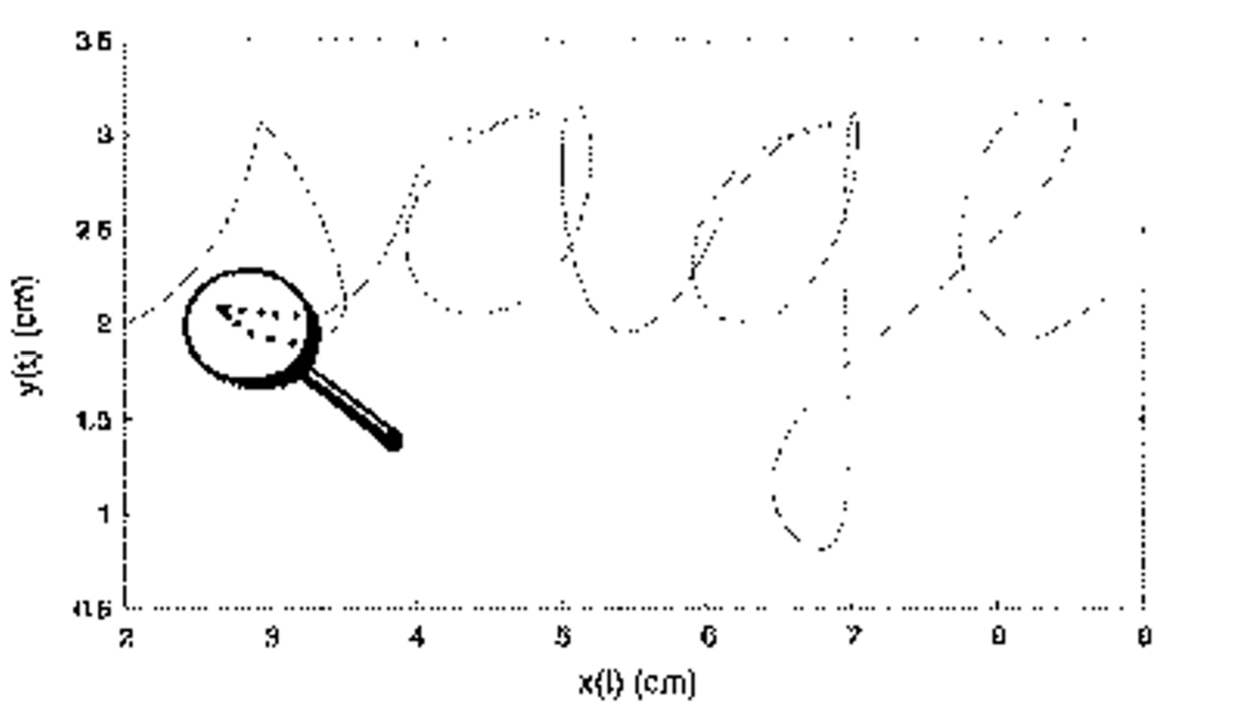
\includegraphics{../../Foto's/Annotation 2020-03-27 163738}
	\caption{x,y coördinaten worden getraceerd in functie van tijd. (\cite{RejeanPlamondon2000})}
	\centering
\end{figure}

Aangezien dit onderzoek primair gebruik zal maken van Off-line Recognition zal dit verder in detail besproken worden.

\section{Off-line recognition}
Het produceren van een performant Off-line Recognition systeem is het doel van tal van onderzoekers in het domein van handschriftherkenning die dit doorheen de jaren proberen te perfectioneren. Handgeschreven teksten zijn een vorm van zelfexpressie, twee dezelfde woorden kunnen een totaal andere betekenis vormen in een verschillende context. Hierdoor kan de achterliggende betekenis van het woord drastisch veranderen. (\cite{GergelyTimar2003})



Zoals reeds besproken maakt Off-line Recognition gebruik van een vooraf geschreven tekst om zo achteraf de tekst te extraheren. Volgens \cite{GergelyTimar2003} kan dit proces dat doorheen verscheidene segmentatie systemen  gebruikt wordt, in een generiek model gegoten worden. 

\begin{figure}[h]
	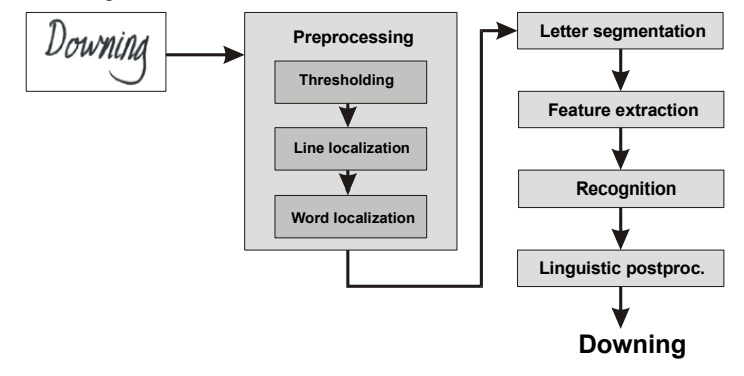
\includegraphics[width=\textwidth,height=\textheight,keepaspectratio]{../../Foto's/Annotation 2020-03-28 141618}
	\captionsetup{justification=centering,margin=2cm}
    \caption{ Het algemeen proces van text extractie via Off-line Recognition. (\cite{GergelyTimar2003})}

	\centering
\end{figure}

\subsection{Preprocessing}

Preprocessing omvat meerdere sub-technieken die toegepast worden vooraleer extractie plaatsvindt. Elk van deze sub-technieken speelt een belangrijke rol in het gehele proces. Zo wordt \textbf{tresholding} toegepast om de effectieve voorgrond-tekst te onderscheiden van de achtergrond. Deze techniek maakt gebruik van een grey-scale versie van het document zodat zwart duidelijk van wit onderscheiden kan worden, zo blijft de tekst geïsoleerd blijft. (\cite{RejeanPlamondon2000}) 

Ter voorbereiding van de karakter segmentatie fase wordt lijn en woordlokalisatie toegepast. Volgens \cite{GergelyTimar2003} helpt deze lokalisatie met het analyseren van de woorden in zijn specifieke context, die op zijn beurt het herkenningspercentage zal verhogen. Het algoritme achter het lokaliseren van deze lijnen is vergelijkbaar met diegene gebruikt in Optical Charachter Recognition. Lijnen worden hierbij gelokaliseerd door het verwerken van de horizontale histogrammen voor het gehele document. Daardoor worden de positie en de graad waar de lijnen een lokaal minimum bereiken gekozen, om zo de plaatsen tussen de lijnen te lokaliseren.  

Eens de lijnen gelokaliseerd zijn kan men vervolgens de woorden lokaliseren. Dit is in principe geen moeilijke taak meer aangezien de onderverdeling van elke lijn gekend is. Men kan door middel van het plaatsen van verticale histogrammen tussen de gekende lijnpunten, de woorden lokaliseren (zie Figuur 2.3). (\cite{GergelyTimar2003}) 

\begin{figure}
\newpage

	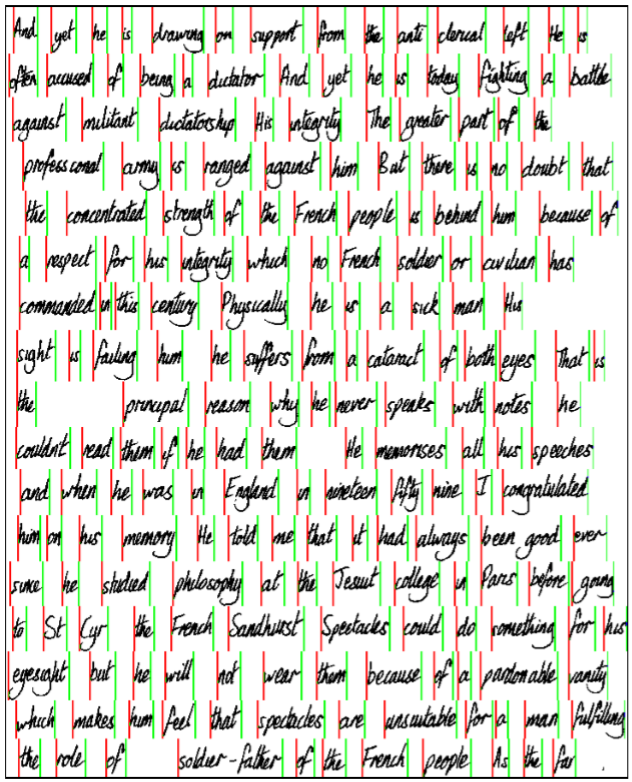
\includegraphics[width=\textwidth,height=\textheight,keepaspectratio]{../../Foto's/line_segmentation_Timar}
	\captionsetup{justification=centering,margin=2cm}
	\caption{Woord segmentatie. (\cite{GergelyTimar2003})}
	\centering
\end{figure}




\subsection{Letter segmentation}
Verdere segmentatie houdt in dat elke letter afgezonderd zal worden. Dit is echter niet zo voor de hand liggend als het lijkt. Het grootste obstakel dat men hier tegenkomt is de variatie in afstand tussen letters. Niet iedereen schrijft letters op dezelfde manier en het kan soms voorvallen dat meerdere karakters overlappen. (\cite{VijayLaxmiSahu2012}) \newline Om karakters op een systematische manier te isoleren wordt Internal Segmentation toegepast. Hierbij probeert men woorden te segmenteren in zijn individuele karakters zonder het gebruik van Feature Extraction. Deze eerste fase houdt geen rekening met eventuele overlappingen en splits elke letter op in een individuele afbeelding. Vervolgens wordt elke afbeelding afzonderlijk geclassificeerd op basis van specifieke kenmerken a.d.h.v. een Hidden Markov Model (HMM).
De cursieve oorsprong van handgeschrift maakt het moeilijk om woorden te segmenteren in karakter afbeeldingen. HMM's helpen om dit probleem op te lossen. 
 (\cite{NafizArica2001}) \newline

HMM’s spelen al jaren een belangrijke rol in het domein van spraak- en gezichtsherkenning. Ondertussen worden deze modellen ook gebruikt bij patroondetectie en vormclassificatie. Deze stochastische modellen kunnen op een zeer efficiënte manier ruis en patroonvariatie in handgeschrift verwerken. Een nadeel van deze aanpak is dat men van de afbeeldingen als invoer verwacht dat deze perfect gesegmenteerd zijn van andere. Aangezien een perfecte aanpak een niet reëel voorkomen is, schat men volgens \cite{Bunke1995} de verwachte herkenningspercentages tussen 74,5 \% en 96.8 \%. 
\subsection{Feature extraction \& Recognition}
Feature extraction is een belangrijk onderdeel van elk patroonherkenning systeem. Dit proces wordt uitgevoerd om de belangrijkste data te extraheren uit de ruwe dataset. Het uiteindelijke doel van dit proces is om een lijst van specifieke “features” van de karakters te bekomen. Met deze aanvullende data kan men vervolgens de herkenningspercentages maximaliseren. Zoals eerder aangereikt verschilt de variëteit in handgeschreven karakters drastisch en kan het extraheren van deze “features” een complexe taak zijn. (\cite{VijayLaxmiSahu2012}) \newline  \newline Men kan karakter features onderscheiden in twee types, namelijk statistische en culturele. Een voorbeeld van statistische feature extraction is Zoning, waarbij men elke karakter afbeelding opdeelt in NxM zones. Hierdoor bekomt men bij bv. een afbeelding van 90 x 60 pixels een onderverdeling van 54 gelijke zones. Vervolgens wordt dit proces herhaald voor elke afbeelding van eenzelfde karakter. Men verkrijgt hierdoor een subset van karakter features waarvan het gemiddelde genomen kan worden. Dit gemiddelde vormt één enkele feature waarde die telkens in die zone geplaats kan worden. (\cite{VijayLaxmiSahu2012})  

Uiteindelijk worden deze features verstuurd naar de recognition engine. Deze retourneert vervolgens een lijst van woorden elk respectievelijk met zijn vertrouwensniveau. Dit niveau stelt voor hoe zeker het algoritme is van zijn voorspelling. (\cite{GergelyTimar2003})

\section{Machine Learning (ML)}
Aangezien in de volgende hoofdstukken machinaal leren aan bod komt, zal hier een kleine inleiding op gegeven worden. 

Machinaal leren (ML) is een concept waarbij men data en een algoritme samen brengt om een specifiek probleem op te lossen. Eens de data en het algoritme getraind zijn krijgt men een model als output. Dit model kan men opnieuw gebruiken met andere data. Het getrainde model geeft inzicht gebaseerd op de nieuwe data. Het bouwen van een ML systeem vergt enige kennis van data science en ML. (\cite{Microsoft2020e})



Volgens \cite{SalimAlHabsib2019} kan men machinaal leren aanpakken op drie manieren: gesuperviseerd leren, ongesuperviseerd leren en semi-gesuperviseerd leren. Gesuperviseerd leren maakt gebruik van gelabelde trainingsdata. Het labelen van deze data neemt zowel tijd als geld in beslag, maar kan op zijn beurt weer geautomatiseerd worden door een neuraal netwerk.  



Semi-gesuperviseerd leren wordt volgens \cite{Zhu2005} beschreven als een speciale vorm van classificatie. Zoals reeds aangereikt, kan gesuperviseerd leren een ingewikkelde en dure manier zijn om een classificatie algoritme op te bouwen. Het labelen van data heeft in de meeste gevallen een vorm van menselijke controle nodig om een acceptabel resultaat te bekomen. Semi-gesuperviseerd leren lost dit probleem op door gebruik te maken van een grote hoeveelheid ongelabelde data, gepaard gaande met een deel gelabelde data. Een vergelijkbare toepassing hiervan, kan men terugvinden bij de Custom Vision service van Azure Cognitive Services. Ongesuperviseerd leren maakt gebruik van ongelabelde data. Het classificeren gebeurt hier door het clusteren van data met gelijkaardige patronen. 

\subsection{Neurale netwerken}

\cite{Kumar2016} beschrijft een  artificieel neuraal netwerk , als een krachtige modelleer tool, die complexe in- en uitgaande relaties kan weergeven en opvangen. De motivatie voor de ontwikkeling van neurale netwerken, stemt af van de nood aan een systeem dat complexe en intelligente taken kan uitvoeren, net zoals de taken uitgevoerd door het menselijk brein. Neurale netwerken komen op twee manieren overeen met het menselijk brein. Ze vergaren leerstof door het leren van vorige transacties en de vergaarde leerstof wordt opgeslagen in de vorm van synaptische gewichten.   


Volgens \cite{Microsoft2020d} worden de volgende types ANN als populairst beschouwd:

\subsubsection{Feedforward neuraal netwerk (FNN)}
Een FNN is één van de meest eenvoudige soort artificiële neurale netwerken. In een FNN mag data maar één richting vloeien, namelijk van de input laag naar de output laag. Data wordt getransformeerd door het gebruik van meerdere lagen. Elke laag bestaat uit een aantal neuronen en is volledig geconnecteerd met al de neuronen in de voorgaande laag. \newpage De laatste volledig geconnecteerde laag stelt de output voor en eveneens de voorspelde labels. (\cite{Microsoft2020d})

\subsubsection{Recurrent neuraal netwerk (RNN)}
Recursieve neurale netwerken worden in een aantal specifieke domeinen gebruikt. Dit type netwerk slaagt de output van een laag op en geeft deze vervolgens terug aan de input laag. Hierdoor bekomt men een vorm van recursie en kan men de uitkomst van een laag op voorhand voorspellen. Deze netwerken worden voornamelijk gebruikt voor complexe taken zoals handschriftherkenning en taalherkenning. (\cite{Microsoft2020d})  
\subsubsection{Convolutioneel neuraal netwerk (CNN)}
Convolutionele neurale netwerken zijn één van de meest doeltreffende types van netwerken, gepaard met een unieke architectuur. Lagen worden in 3 dimensies opgebouwd: breedte, hoogte en diepte. 

Neuronen in de ene laag connecteren partieel met al de neuronen in de volgende laag. De finale output laag wordt gereduceerd tot een enkelvoudige vector van waarden die het vertrouwensniveau van de voorspelling weergeeft. Convolutionele neurale netwerken worden voornamelijk gebruikt bij video en afbeelding herkenning. (\cite{Microsoft2020d}) 






\section{Cloud computing providers}
Wanneer men dus uiteindelijk handschriftherkenning in een project wenst te integreren zijn er meerdere mogelijkheden. Men kan gebruik maken van een Cloud computing platform dat services zoals tekstherkenning en extractie aanbiedt, maar er is natuurlijk ook de optie om een open source framework zoals Tenserflow of Theano te gebruiken. Bij deze open source optie wordt er verwacht dat men het neurale netwerk/model volledig zelfstandig opbouwt en een eigen inbreng van trainingsdata voorziet. In sommige gevallen kan dit een voordeel zijn, wanneer er bv. een zeer specifiek model nodig is. Cloud gebaseerde oplossingen hebben hierbij het voordeel dat ze een model gebruiken dat getraind is met data verzameld door de provider. Verscheidene providers laten het toe om zelf nog extra trainingsdata in te brengen in het model, zoals bv. de Custom Vision service van Microsoft Azure. 



In het domein van Cloud Computing zijn er dus enkele marktleiders die een forse voorsprong hebben door middel van de hoeveelheid data die zij door de jaren heen hebben verzameld. Dit onderzoek maakt voornamelijk gebruik van de services die Microsoft Azure te bieden heeft, maar er zullen in de volgende hoofdstukken nog enkele andere alternatieven besproken worden die een gelijkaardig pakket aanbieden. 

\section{\IfLanguageName{dutch}{Microsoft Azure}{Azure}}

Microsoft Azure is een uitgebreide set van cloud services die helpt bij het organiseren en het aanpakken van uitdagingen die zich voordoen op grootschalige niveaus. Deze uitdagingen worden typisch gerealiseerd door middel van cloud computing.  Wanneer iemand niet beschikt over de nodige server of opslagcapaciteiten die zich kunnen voordoen bij sommige uitdagingen, dan kan men opteren voor cloud computing.  Hierbij kan men bij providers zoals Azure, gebruik maken van de cloud om data op te slagen. Cloud computing platformen zoals Azure worden gerealiseerd door meerdere datacentrales op een globaal niveau. Hierdoor kan men wereldwijd op een betrouwbare manier toegang bieden tot verscheidene services die beschikbaarheid en betrouwbaarheid van data realiseren. (\cite{Microsoft2020a}) \newline
\newline
Volgens \cite{VaibhavAGhandi1999} kan men cloud computing opdelen in verschillende service modellen. 





\subsection{Software as a Service (SaaS)}
Software as a Service is een software gedistribueerd model waarin applicaties door een service provider gehost worden. De betalingsmethode voor SaaS volgt een subscriptie gebaseerd model. Hierdoor kunnen organisaties de focus leggen op hun core business zonder zich bezig te houden met infrastructuur management. (\cite{ManishGodse2009})
\subsection{Platform as a Service (PaaS)}
Platform as a Service biedt bedrijven een digitaal platform voor ontwikkeling en inzet van hun eigen applicaties en services. Hierdoor elimineert men de nood aan het onderhouden van servers, het programmeren van software en het opstellen van interne veiligheid protocollen. (\cite{Wright2019})
\subsection{Infrastructure as a Service (IaaS)}
Infrastructure as a service is de bundeling van hardware en geassocieerde software geleverd als een service. Deze hardware kan bestaan uit servers, opslag en of netwerk toepassingen. Meegeleverde software kan gaan van besturingssystemen, virtualisatie technologieën of file systemen. Bij IaaS is de provider enkel verantwoordelijk voor het operationeel houden van de data centers. Klanten zijn zelf verantwoordelijk voor het opstellen en het onderhouden van hun software services. (\cite{Bhardwaj2010})
\begin{figure}[h]

	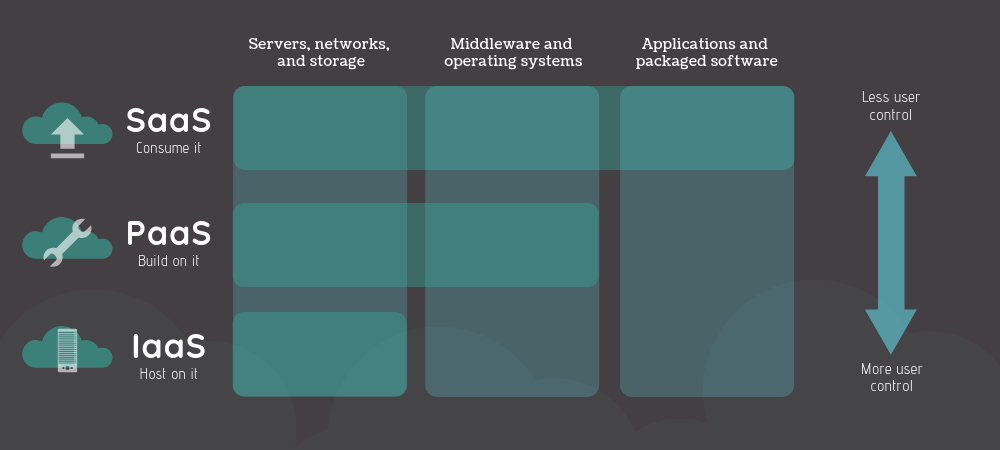
\includegraphics[width=\textwidth,height=\textheight,keepaspectratio]{../../Foto's/Cloud-Models-Graphics}
	\captionsetup{justification=centering,margin=2cm}
	\caption{SaaS,IaaS,PaaS. (\cite{Wright2019})}
	\centering
\end{figure}
\section{\IfLanguageName{dutch}{Azure Cognitive Services}{Azure Cognitive Services}}
Azure cognitive services geeft ontwikkelaars de kans om op een eenvoudige wijze artificiële intelligentie toe te voegen aan hun project zonder enige voorkennis te hebben van machinaal leren en/of data science. Toepassingen van cognitive services gaan van het analyseren en herkennen van objecten in afbeeldingen tot het herkennen van emoties op gezichten in realtime.  Een cognitive service levert deels of de volledige componenten die nodig zijn in een toepassing die gebruik maakt van machinaal leren. Deze componenten kunnen bestaan uit bv. data, het algoritme of een vooraf getraind model. Een service zoals deze verwacht dat de gebruiker generieke info over de dataset meelevert.  (\cite{Microsoft2020b}) \newline \newline



Azure cognitive services kan geclassificeerd worden als een Software as a Service (SaaS), omvat een groep van services die onmiddellijk beschikbaar zijn voor deployment en kunnen opgedeeld worden in de volgende categorieën:

\begin{itemize}
	\item \textbf{Decision:} Bouwt apps die aanbevelingen geven voor het maken van efficiënte en geïnformeerde beslissingen.
	\item \textbf{Language:} Zorgt ervoor dat men taal kan verwerken met voorgebouwde scripts, die emoties evalueren en leren wat een gebruiker juist wenst.
	\item \textbf{Search:} Voegt Bing Search API’s toe aan apps en geven de mogelijkheid om miljarden webpagina’s, afbeeldingen en video's te doorzoeken met één enkele API.
	\item \textbf{Speech:} Transformeert gesproken tekst naar digitale tekst en vertaalt één taal naar een ander samen met spraak verificatie en herkenning.
	\item \textbf{Vision:} Herkent, identificeert, indexeert en onderhoudt foto's, video's en digitale inkt toepassingen.
\end{itemize}
Sommige van deze services maken het mogelijk om zelf training data mee te geven om vervolgens een model te trainen. Hierdoor kan men het model uitbreiden door gebruik te maken van de data die de service levert samen met de data die de gebruiker meelevert. Wanneer men zelf data meelevert, kan het voorvallen dat deze data nog op een specifieke manier gelabeld moet worden conform met de service. Door zelf data mee te geven kan je de service vormen naar de noden van de gebruiker. (\cite{Microsoft2020b})



\section{\IfLanguageName{dutch}{Azure Computer Vision framework}{Azure Computer Vision framework}}
Computer vision biedt een aantal services die afgedrukte of handgeschreven tekst detecteren en extraheren. Dit kan in verschillende situaties toegepast worden, zoals het maken van notities, inscannen van medische dossiers of bij beveiliging en bankieren. Voor het herkennen van tekst levert het Computer Vision Framework drie verschillende API’s elk geoptimaliseerd voor een specifieke toepassing. (\cite{Microsoft2020c})

\subsection{Read API}
De Read API kan tekst in een afbeelding detecteren met behulp van de nieuwste herkenningsmodellen van computer vision, en zet geïdentificeerde tekst om in een karakterstroom. Deze API is voornamelijk geoptimaliseerd voor afbeeldingen die veel tekst hebben of
met een bepaald aantal visuele ruis. Voor elke lijn tekst wordt eveneens beslist welk herkenningsmodel gebruikt zal worden. Hierdoor ondersteunt de API geprinte en handgeschreven tekst. De Read API voert de herkenningsalgoritmen asynchroon uit omdat men bij data intensieve documenten een langere tijd nodig heeft tot men een resultaat verkrijgt. (\cite{Microsoft2019})
\newline
\newline
De leesoperatie houdt de originele lijn groeperingen van herkende woorden bij in zijn output. Elke lijn heeft zijn eigen coördinaten. Respectievelijk heeft elk woord in deze lijn ook zijn specifieke coördinaten. Wanneer een herkend woord een lage vertrouwens niveau heeft wordt dit percentage per woord meegeleverd. (\cite{Microsoft2019})
\subsection{OCR API}
Men kan in grote lijnen de OCR API gelijkstellen aan de Read API, echter voert deze API zijn operaties synchroon uit en zijn deze niet geoptimaliseerd voor data intensieve documenten. Hiervoor maakt de OCR API gebruik van een ouder herkenningsmodel maar is deze ook compatibel met meerdere talen. 

Wanneer nodig kan OCR de rotatie van specifiek herkende tekst aanpassen door middel van de afbeelding te draaien op zijn horizontale as (ziet figuur 2.5).  
\begin{figure}[h]
	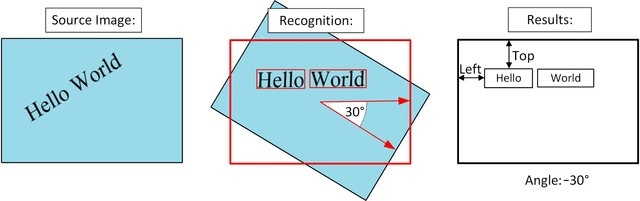
\includegraphics[width=\textwidth,height=\textheight,keepaspectratio]{../../Foto's/vision-overview-ocr}
		\captionsetup{justification=centering,margin=2cm}
	\caption{Rotatie correctie van een woord via de OCR API. (\cite{Microsoft2019})}
	\centering
\end{figure}
\subsection{Recognize text API}
De Recognize Tekst API is in zekere zin gelijkaardig aan dat van OCR, maar verwerkt zijn operaties asynchroon en maakt gebruik van geüpdatete herkenningsmodellen. Deze API heeft echter enkele limitaties. De accuraatheid van deze operaties is grotendeels afhankelijk van de kwaliteit van de gebruikte afbeeldingen. De volgende factoren kunnen de accuraatheid beïnvloeden: 
\begin{itemize}
	\item Wazige afbeeldingen.
	\item  Handgeschreven of cursieve tekst.
	\item Artistieke font keuzes.
	\item Kleine tekstgrote.
	\item Complexe achtergronden, schaduwen over tekst.
\end{itemize}
(\cite{Microsoft2019})


\section{\IfLanguageName{dutch}{Google Cloud Platform (GCP)}{Google}}
Google Cloud Platform (GCP) biedt net zoals Microsoft Azure services voor opslag, analyse, big data en machine learning op een globaal niveau. Google realiseert dit door hun grootschalig netwerk van datacenters verspreid over 22 regio’s. Door de spreiding van deze locaties kan men efficiënte en betrouwbare connectie met de cloud verzekeren. 


Men kan de services die Google levert opdelen in enkele omvattende categorieën:
\begin{itemize}
	\item \textbf{Compute engine:} De compute engine levert flexibele virtuele machines die draaien op de Google datacenters. 
	\item \textbf{Storage \& Databases:} Voorziet globale toegang tot verschillende opslag architecturen op enterprise niveau.  
	\item \textbf{Machine learning:} Maakt het mogelijk voor developers om machine learning in een project te integreren en eveneens over te gaan naar een productieomgeving.  \newpage
	\item \textbf{Big data:} Opslag en analyse mogelijkheden van grote hoeveelheden data, gepaard met data warehouse integratie en stream analytics. 
	\item \textbf{Developer tools:} Voorziet pipelines en automatisatie van deployment in een productie omgeving.
	
\end{itemize}
\begin{figure}[h]
	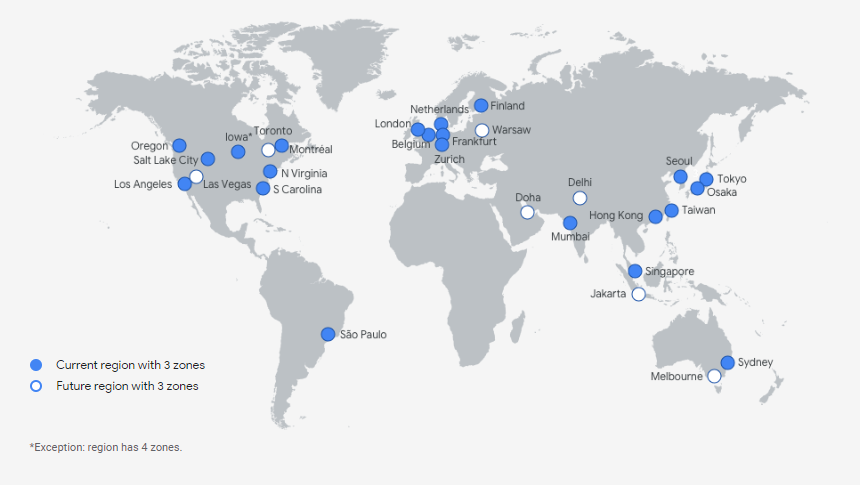
\includegraphics[width=\textwidth,height=\textheight,keepaspectratio]{../../Foto's/Google cloud locations}
		\captionsetup{justification=centering,margin=2cm}
	\caption{Google datacenters. (\cite{Google2020a})}
	\centering
\end{figure}


Vergelijkbaar met Azure Cognitive Services heeft GCP een gelijkaardig machine learning platform, namelijk AI hub. De Google Cloud AI Hub is een gehoste opslagplaats waarbij men kant-en-klare AI toepassingen kan implementeren, en end-to-end AI pipelines kan opzetten. AI Hub biedt ook professionele deelmogelijkheden waarmee men AI toepassingen privé kan hosten. (\cite{Google2020b})



Naar aanleiding van dit onderzoek worden meerdere toepassingen besproken waarmee handschriftherkenning gerealiseerd kan worden. De oplossing die Google hier namelijk voor voorziet is Google Vision AI, meer specifiek de Cloud Vision API. 

Google Vision AI biedt meerdere opties aan om computer visie modellen te integreren in applicaties of in websites. Men kan deze opties verder onderverdelen in drie categorieën: 
\begin{itemize}
	\item Auto ML Vision
	\item Cloud Vision API
	\item Cloud Vision product search
\end{itemize}
(\cite{Google2020c})


\subsection{Cloud Vision API}
De Google Cloud Vision API biedt een verzameling van technologieën die men kan gebruiken om de inhoud van afbeeldingen te analyseren. Hiervoor kan men gebruik maken van een zelf getraind ML model of één van de vele vooraf getrainde modellen die de API aanbiedt. Door gebruik te maken van AutoML Vision kan men naast de vooraf gedefinieerde labels, zelf specifieke labels toevoegen. Hierdoor kan men een domein specifiek model opbouwen. Toepassingen die gebruik maken van deze vooraf getrainde modellen omvatten, maar zijn niet gelimiteerd tot: afbeelding classificatie, object detectie, geprinte en handgeschreven tekstherkenning, gezichtsherkenning, product logo identificatie. (\cite{Google2020d})


De Vision API kan tekst in afbeeldingen detecteren en extraheren. Net zoals het Computer Vision framework van Microsoft, maakt Google ook gebruik van de OCR technologie om de achterliggende logica van karakter herkenning te realiseren. Er zijn namelijk 2 annotatie technieken die de Vision API ondersteunt: 

\begin{itemize}
	\item \textbf{TEXT\_DETECTION:} Deze annotatie techniek wordt voornamelijk gebruikt voor het extraheren van geprinte tekst. Hiermee kan men bv. de tekst van een verkeersbord herkennen.  
	\item \textbf{DOCUMENT\_TEXT\_DETECTION:} Wordt ook gebruikt voor tekst extractie maar is geoptimaliseerd voor documenten en handgeschreven teksten. 
\end{itemize}


Beide technieken worden getriggerd bij aanvang van een REST request. De request body bestaat uit een JSON string. In deze string wordt een base64 gecodeerde afbeelding meegegeven samen met de gewenste annotatie techniek. Wanneer de request als succesvol wordt beschouwd door de server, dan retourneert deze een HTTP status code 200 OK. 


De status code 200 geeft aan dat het verzoek geslaagd is, gepaard met deze status code wordt ook een response body geretourneerd in JSON formaat. In deze response wordt de gedetecteerde zin meegegeven, de geschatte taal en de coördinaten van waar de zin zich precies bevindt in de afbeelding. De Vision API voorziet ook de optie om rechtstreeks een afbeelding van Google Cloud of het web mee te geven bij de request. (\cite{Google2020e}) 


Op figuur 2.7 ziet men een voorbeeld van hoe een JSON request body opgebouwd wordt. 


Beide types ondersteunen de integratie van één of meerdere taal hints. Deze hints specifiëren de taal van de tekst die voorkomt in de meegegeven afbeelding. Dit kan in de sommige gevallen de snelheid van extractie verhogen. Meestal wanneer men dit niet specifieert bekomt men betere resultaten, aangezien de API zelf automatisch de taal detecteert. Het kan zelfs voorvallen dat een foutieve taal hint de herkenning kan hinderen. 
\begin{figure}[h]
	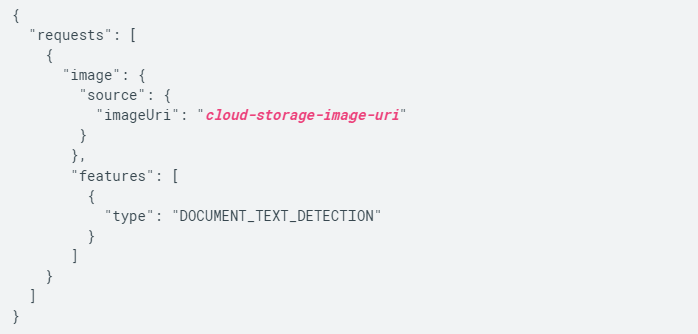
\includegraphics[width=\textwidth,height=\textheight,keepaspectratio]{../../Foto's/vision OCR request body Google}
		\captionsetup{justification=centering,margin=2cm}
	\caption{Text extractie request body. (\cite{Google2020e})}
	\centering
\end{figure}

\section{Amazon Web Services (AWS)}
Amazon Web Service (AWS) is de derde grote tegenhanger in het domein van Cloud Computing, naast Microsoft Azure en Google Cloud.  



AWS maakt hun services wereldwijd beschikbaar op meerdere locaties. Deze locaties bestaan uit verschillende individuele regio's en zones. Elke regio is verder opgedeeld in geïsoleerde locaties gekend als “beschikbaarheid zones”. AWS laat het toe om meerdere resources zoals instanties van AWS services of data, te deployen op meerdere locaties. Deze resources worden niet over verschillende regio's gedupliceerd, tenzij men dit expliciet specifieert. Elke regio is volledig zelfstandig en isoleert zich volledig van andere regio’s. Hierdoor bekomt men een hoge graad van fout tolerantie en stabiliteit over het netwerk. (\cite{Amazon2020a})



AWS levert net zoals de concurrentie, tal van Cloud Computing services. Elk van deze service kan gebundeld worden in een cluster van services: 


\begin{itemize}
	\item \textbf{Analytics}
	\item \textbf{Application Integration}
	\item \textbf{Compute}
	\item \textbf{Database}
	\item \textbf{Internet of Things}
	\item \textbf{Machine Learning}
	\item \textbf{Containers}
\end{itemize}


\subsection{Amazon Rekognition}
Amazon Rekognition valt onder de AWS Machine Learning cluster maakt het mogelijk om op een eenvoudige wijze video en afbeelding analyse toe te voegen aan een applicatie. Wanneer men een afbeelding of een video meegeeft in een extractie request naar de Rekognition API, dan kan de API op een accurate manier objecten, mensen, tekst en activiteiten detecteren. Er is ook de mogelijkheid om net zoals bij Google Cloud Vision, custom labels mee te geven, om een model te maken dat gespecifieerd is aan de noden van de klant. (\cite{Amazon2020b})


De Rekognition API kan tekst in afbeeldingen en video's detecteren, en deze vervolgens converteren naar machinale tekst. Men kan een afbeelding aan een request meegeven in de vorm van een base64 gecodeerde string of een Amazon S3 object (zie figuur 2.8). Amazon S3 is een opslag service aangeboden door AWS, waar men key–value paren van objecten in kan opslagen. Deze objecten kan men rechtstreeks meegeven aan een API request en is niet gelimiteerd tot enkel afbeeldingen. (\cite{Amazon2019})

\begin{figure}[h]
	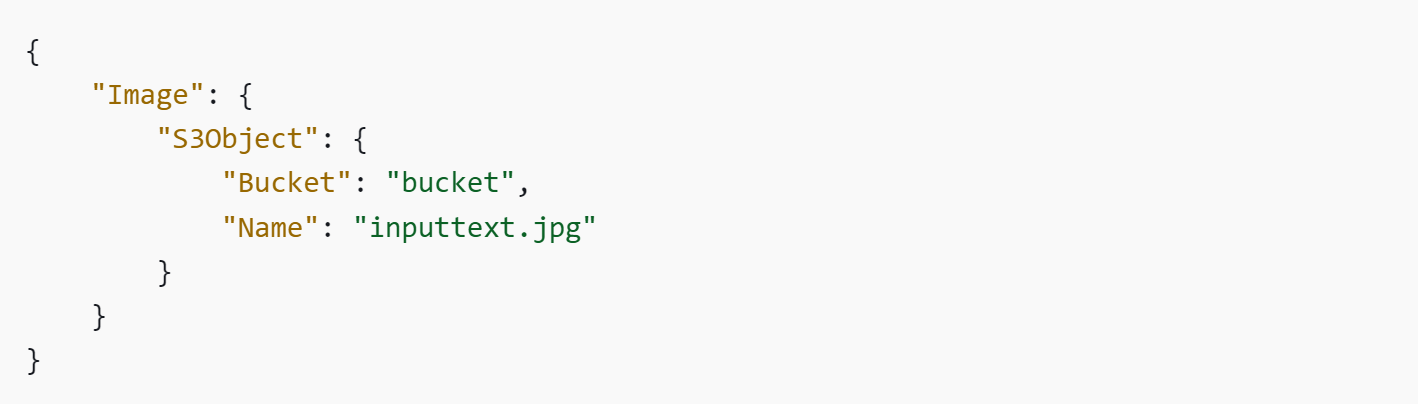
\includegraphics[width=\textwidth,height=\textheight,keepaspectratio]{../../Foto's/AWS text detection request}
	\captionsetup{justification=centering,margin=2cm}
	\caption{Text extractie request body. (\cite{Amazon2019})}
	\centering
\end{figure}



Vervolgens retourneert de API een JSON response waarin de herkende woorden samen met hun vertrouwensniveau en positie weergeven worden. 

\section{Eerder uitgevoerd onderzoek}
Zoals aangereikt in de inleiding is dit onderzoek gebaseerd op een recent onderzoek uitgevoerd door Vectr. Consulting in samenwerking met de Christelijke Mutualiteit. Hierbij ontwikkelde zij een bot die automatisch doktersgeschrift op Belgische doodsaktes met een accuraatheid van 47 \% correct voorspelde. Hiervoor maakten zij gebruik van het machine learning framework Tenserflow van Google, gepaard met een convolutioneel neuraal netwerk ontwikkeld door H. Scheidl. De data gebruikt in het trainen van dit neuraal netwerk werd verzameld gedurende 6 jaar. Finale resultaten van dit onderzoek tonen aan dat 47\% van de testset correct gelabeld werd door het neuraal netwerk. Dit percentage is zeer gevoelig aan de kwaliteit van de preprocessing op de data en de segmentatie van woorden in karakters. Uit dit onderzoek kon men uiteindelijk concluderen dat het herkennen van doktersgeschrift zeker haalbaar is met een degelijk getraind neuraal netwerk. 



%%=============================================================================
%% Methodologie
%%=============================================================================

\chapter{\IfLanguageName{dutch}{Methodologie}{Methodology}}
\label{ch:methodologie}

%% TODO: Hoe ben je te werk gegaan? Verdeel je onderzoek in grote fasen, en
%% licht in elke fase toe welke stappen je gevolgd hebt. Verantwoord waarom je
%% op deze manier te werk gegaan bent. Je moet kunnen aantonen dat je de best
%% mogelijke manier toegepast hebt om een antwoord te vinden op de
%% onderzoeksvraag.

Na een adequate hoeveelheid informatie vergaard te hebben bij het literatuuronderzoek, was het vervolgens mogelijk om het praktische deel van dit onderzoek uit te voeren. Uit de literatuurstudie kon vastgesteld worden dat handschriftherkenning op meerdere manieren gerealiseerd kon worden. Cloud computing voorziet een eenvoudige implementatie met behulp van vooraf getrainde modellen, maar komt met additionele transactiekosten. Een open source machine learning framework zoals Tenserflow kan in deze situatie een zeer effectieve oplossing bieden. 


Men kan zoals gezien bij het onderzoek uitgevoerd door Vectr. Consulting, een zeer specifiek model opbouwen met zelf vergaarde data. Dit vormde echter een probleem bij dit onderzoek aangezien handgeschreven doktersbriefjes als een nogal confidentiële vorm van documenten worden bezien. Verder ligt de hoeveelheid data nodig om een toelaatbaar resultaat te bekomen hoog, dit zou enige tijd vergen om deze te bekomen. 


Een reële aanpak was dus om gebruik te maken van één van deze Cloud computing oplossingen, alsook te observeren hoe een model getraind met een generieke dataset reageert op doktersgeschrift.

\newpage
\subsection{Gebruikte technologie}
Aangezien ik momenteel een stage volg waar het gebruik van de Microsoft Azure Cloud centraal staat, leek het een interessante keuze om bij dit onderzoek gebruik te maken van de Computer Vision API van Azure Cognitive Services, meer bepaald de Read API. Hierbij kan zoals besproken in hoofdstuk 2.8 van het literatuuronderzoek, de API gebruikt worden om handgeschreven teksten te achterhalen van afbeeldingen. Daarom werd in een volgend hoofdstuk de onderdelen van deze API tot in detail besproken, samen met de software implementatie die hiermee communiceert.
\subsection{Test cases}
Om aan te tonen hoe de ontwikkelde software presteert, werden enkele test cases opgesteld. Bij elke test case werd een specifiek obstakel, dat zou kunnen voorvallen bij extractie, getest. Zo wordt bij de eerste test een afbeelding van een doktersvoorschrift gebruikt dat een lager dan normale resolutie heeft. Hierdoor worden de limitaties van de API op proef gesteld aangezien deze geen minimum resolutie definieert.


Een tweede meer fundamenteel gerichte test werd uitgevoerd om de gemiddelde accuraatheid van de API te testen. Hierbij werd er een extractie request afgevuurd op een aantal doktersbriefjes van hetzelfde type om zo inzicht te krijgen in hoe de API reageert op een normale workload. De teruggekregen data van deze request wordt achteraf samengebracht en weergegeven bij de resultaten.


Een derde en laatste test werd uitgevoerd om te testen of het uiterlijk van een voorschrift invloed heeft op het extractie resultaat. Verschillende voorschriften kunnen een vorm van hulplijnen hebben om de schrijver te helpen. Dit brengt mogelijks voor- en nadelen met zich mee en kan het beoogde resultaat beïnvloeden. 
\subsection{Resultaten}
Uiteindelijk werd de bekomen data resulterend uit de test cases in een grafiek gegoten, waarbij de accuraatheid en payload van elke extractie request vergeleken werd. De uitkomst van deze resultaten bepaalde eveneens de bekomen conclusie van dit onderzoek en geeft wel degelijk aan of het mogelijk is om doktersgeschrift te extraheren van een voorschrift. Eveneens geeft dit ook een reëel inzicht over de meerwaarde die deze oplossing kan bieden op lange termijn. 

\chapter{Cognitive services computer vision}
Vooraleer men de Computer Vision API kan gebruiken moet men in het bezit zijn van een lopende Microsoft Azure subscriptie. Deze subscriptie komt in een aantal verschillende opties en varieert drastisch in prijs en beschikbare noden. In figuur 4.1 worden de Azure subscriptie mogelijkheden duidelijk weergegeven met hun specifieke karakteristieken.  Elke subscriptie type heeft zijn plaats en voordeel binnen de Azure cluster.   

Aangezien studenten recht hebben op een gratis 30 dagen proefabonnement met een kredietlimiet van € 130, volstaat een Visual Studio subscriber abonnement voor dit onderzoek.  Zoals weergegeven op figuur 4.1, zijn deze individuele abonnementen ook beschikbaar met een kredietscore van € 45 en € 85. Deze credits zijn gedurende de loop van een volledige maand beschikbaar. (\cite{Microsoft2020f}) 



Vervolgens is er de mogelijkheid om één van de vele beschikbare services aan te vragen die Microsoft Azure te bieden heeft. Credits worden automatisch afgenomen van het gebruikersaccount, in functie van de hoeveelheid calls uitgevoerd per service.  
\begin{figure}
	\newpage
	
	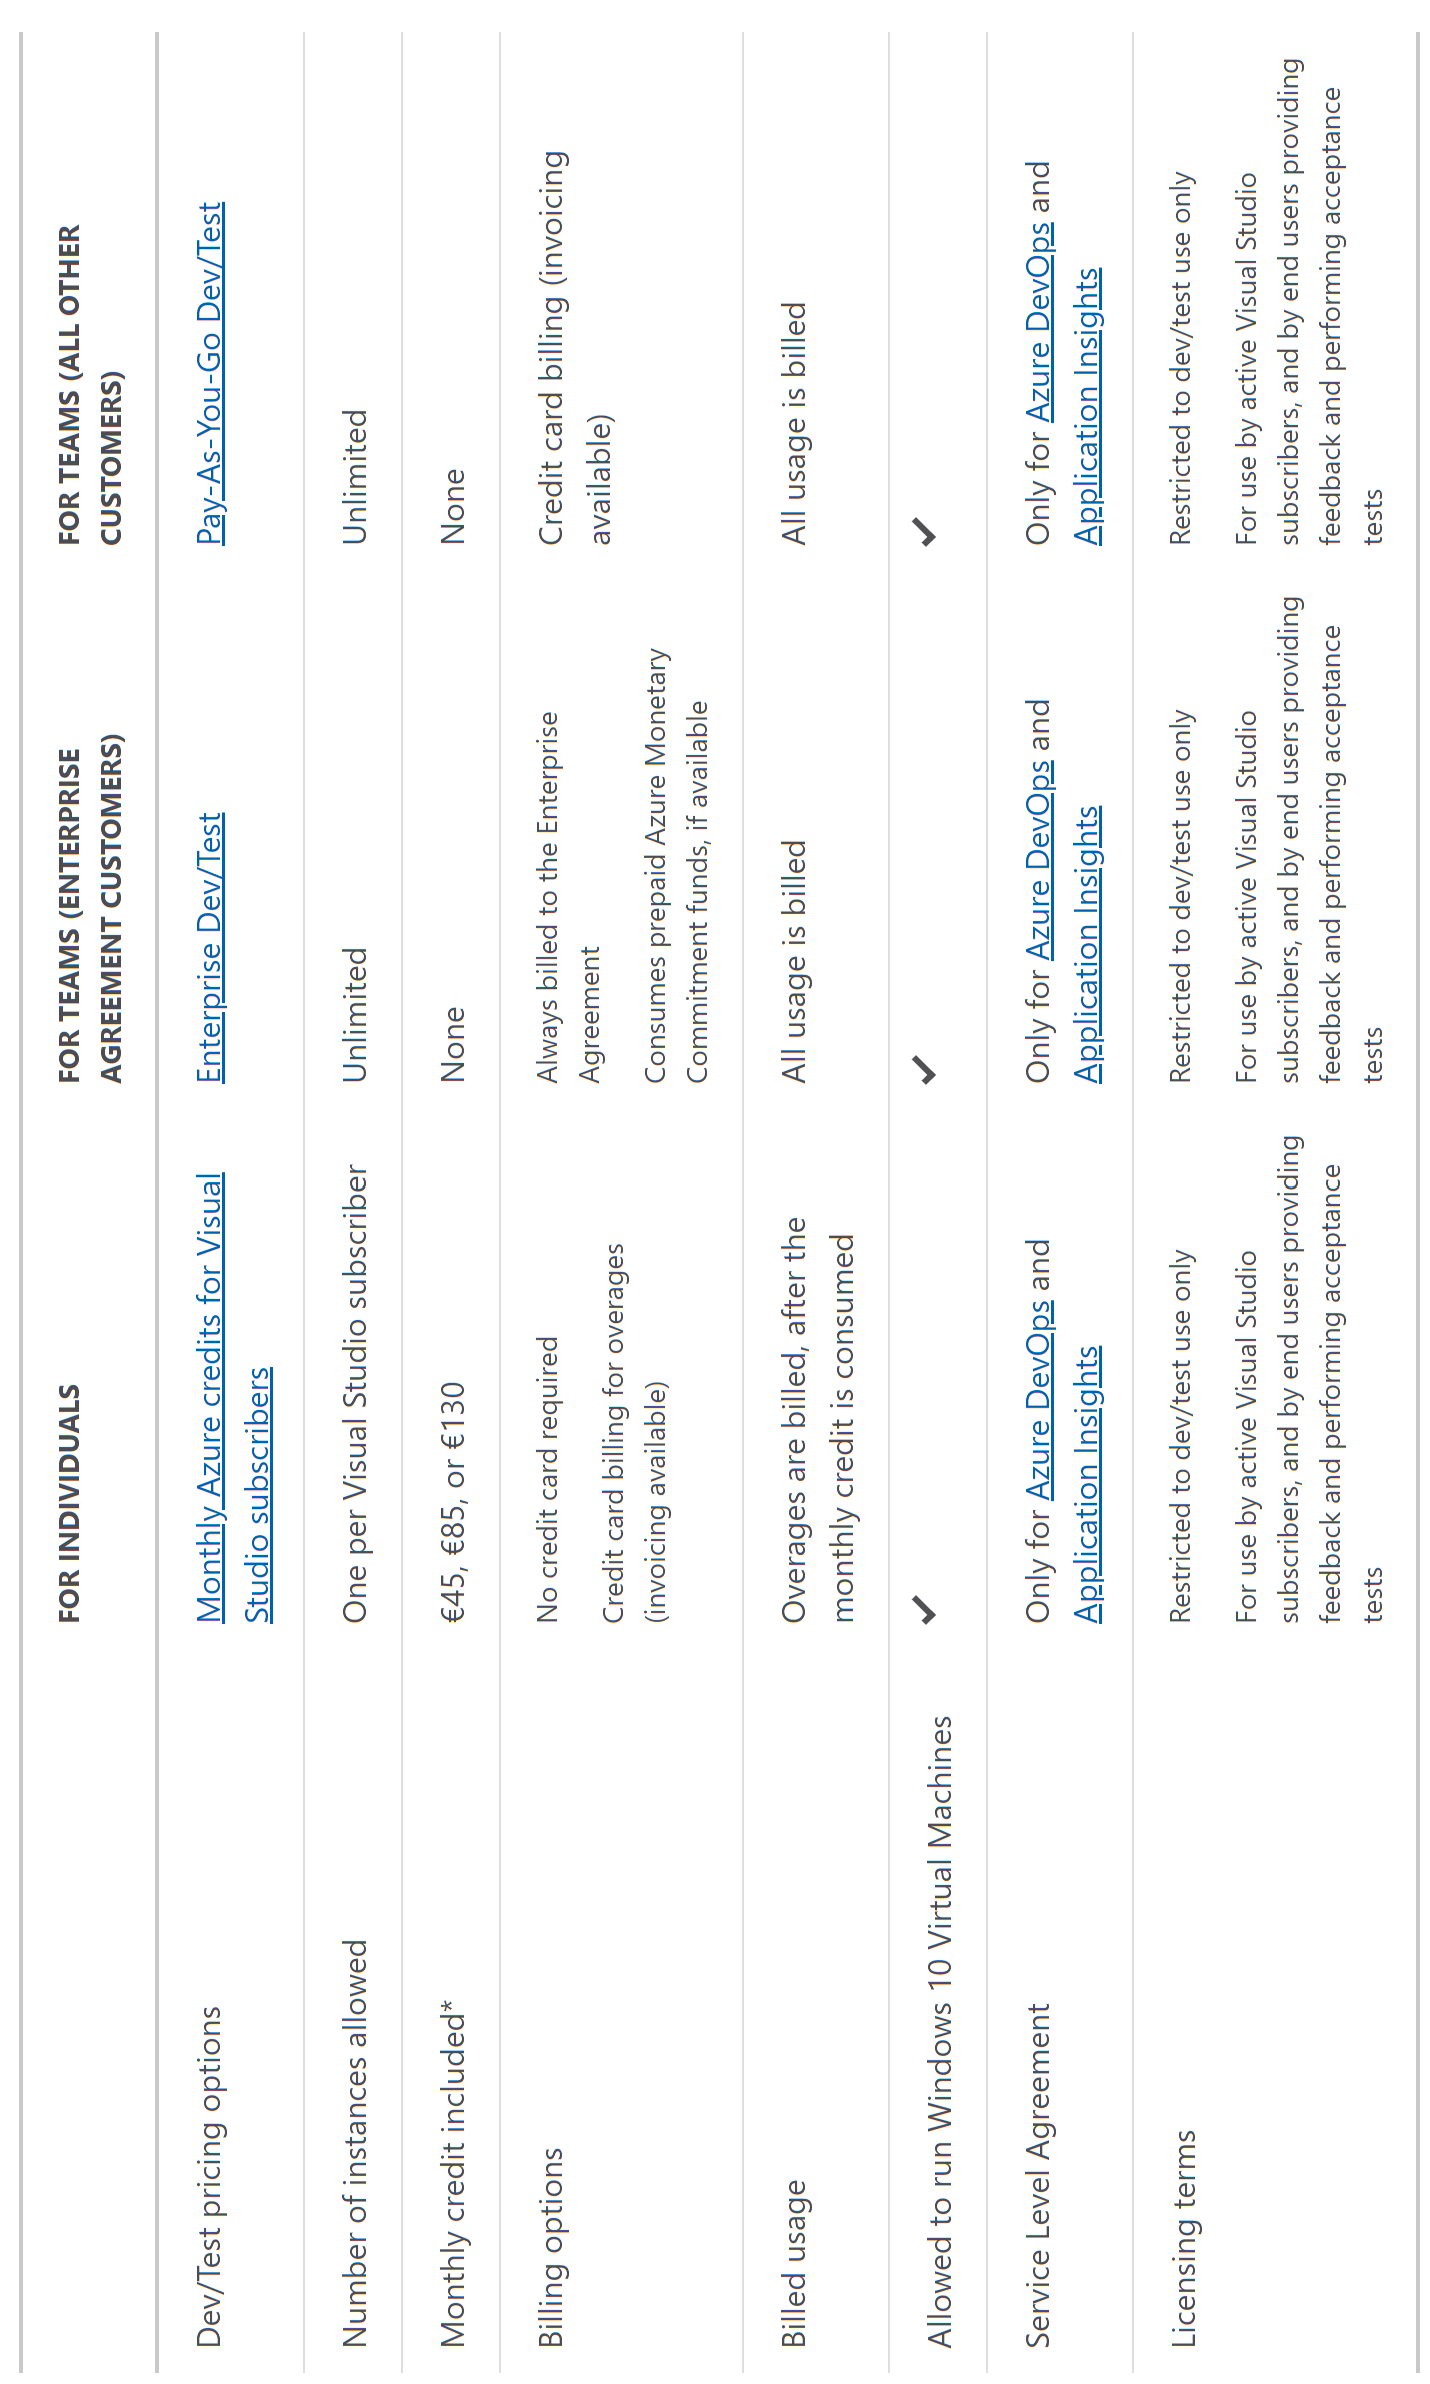
\includegraphics[width=\textwidth,height=\textheight,keepaspectratio]{../../Foto's/azure-pricing-tiers} 
	\captionsetup{justification=centering,margin=2cm}
	\caption{Azure Dev/Test prijzen. (\cite{Microsoft2020f})}
	\centering
\end{figure}

\subsection{Opzet API}
In de volgende sectie wordt de configuratie en opzet van een appservice, meer bepaald de Computer Vision API, in chronologische volgorde doorlopen en besproken. Hierbij wordt er inzicht gegeven in de mogelijke limitaties van de API en eveneens de verbonden transactiekosten. Na de opzet van deze API is het mogelijk om deze aan te roepen vanuit een software implementatie die in de volgende sectie besproken wordt. 


\newpage Een service kan men aanvragen via de Azure marketplace, hier wordt er een overzicht weergeven van de verschillende categorieën van services. De Computer Vision API valt onder de categorie: ‘AI + Machine Learning’ en wordt beschouwd als een Cognitieve Service. (\cite{Microsoft2020c}) 



De eerste stap is het navigeren naar de marketplace om vervolgens Computer Vision te selecteren. Na deze selectie krijgt men de optie aangeboden om een instantie van deze service aan te maken, gepaard gaande met de configuratie mogelijkheden zichtbaar op figuur 4.2   
\begin{figure}[h]
	
	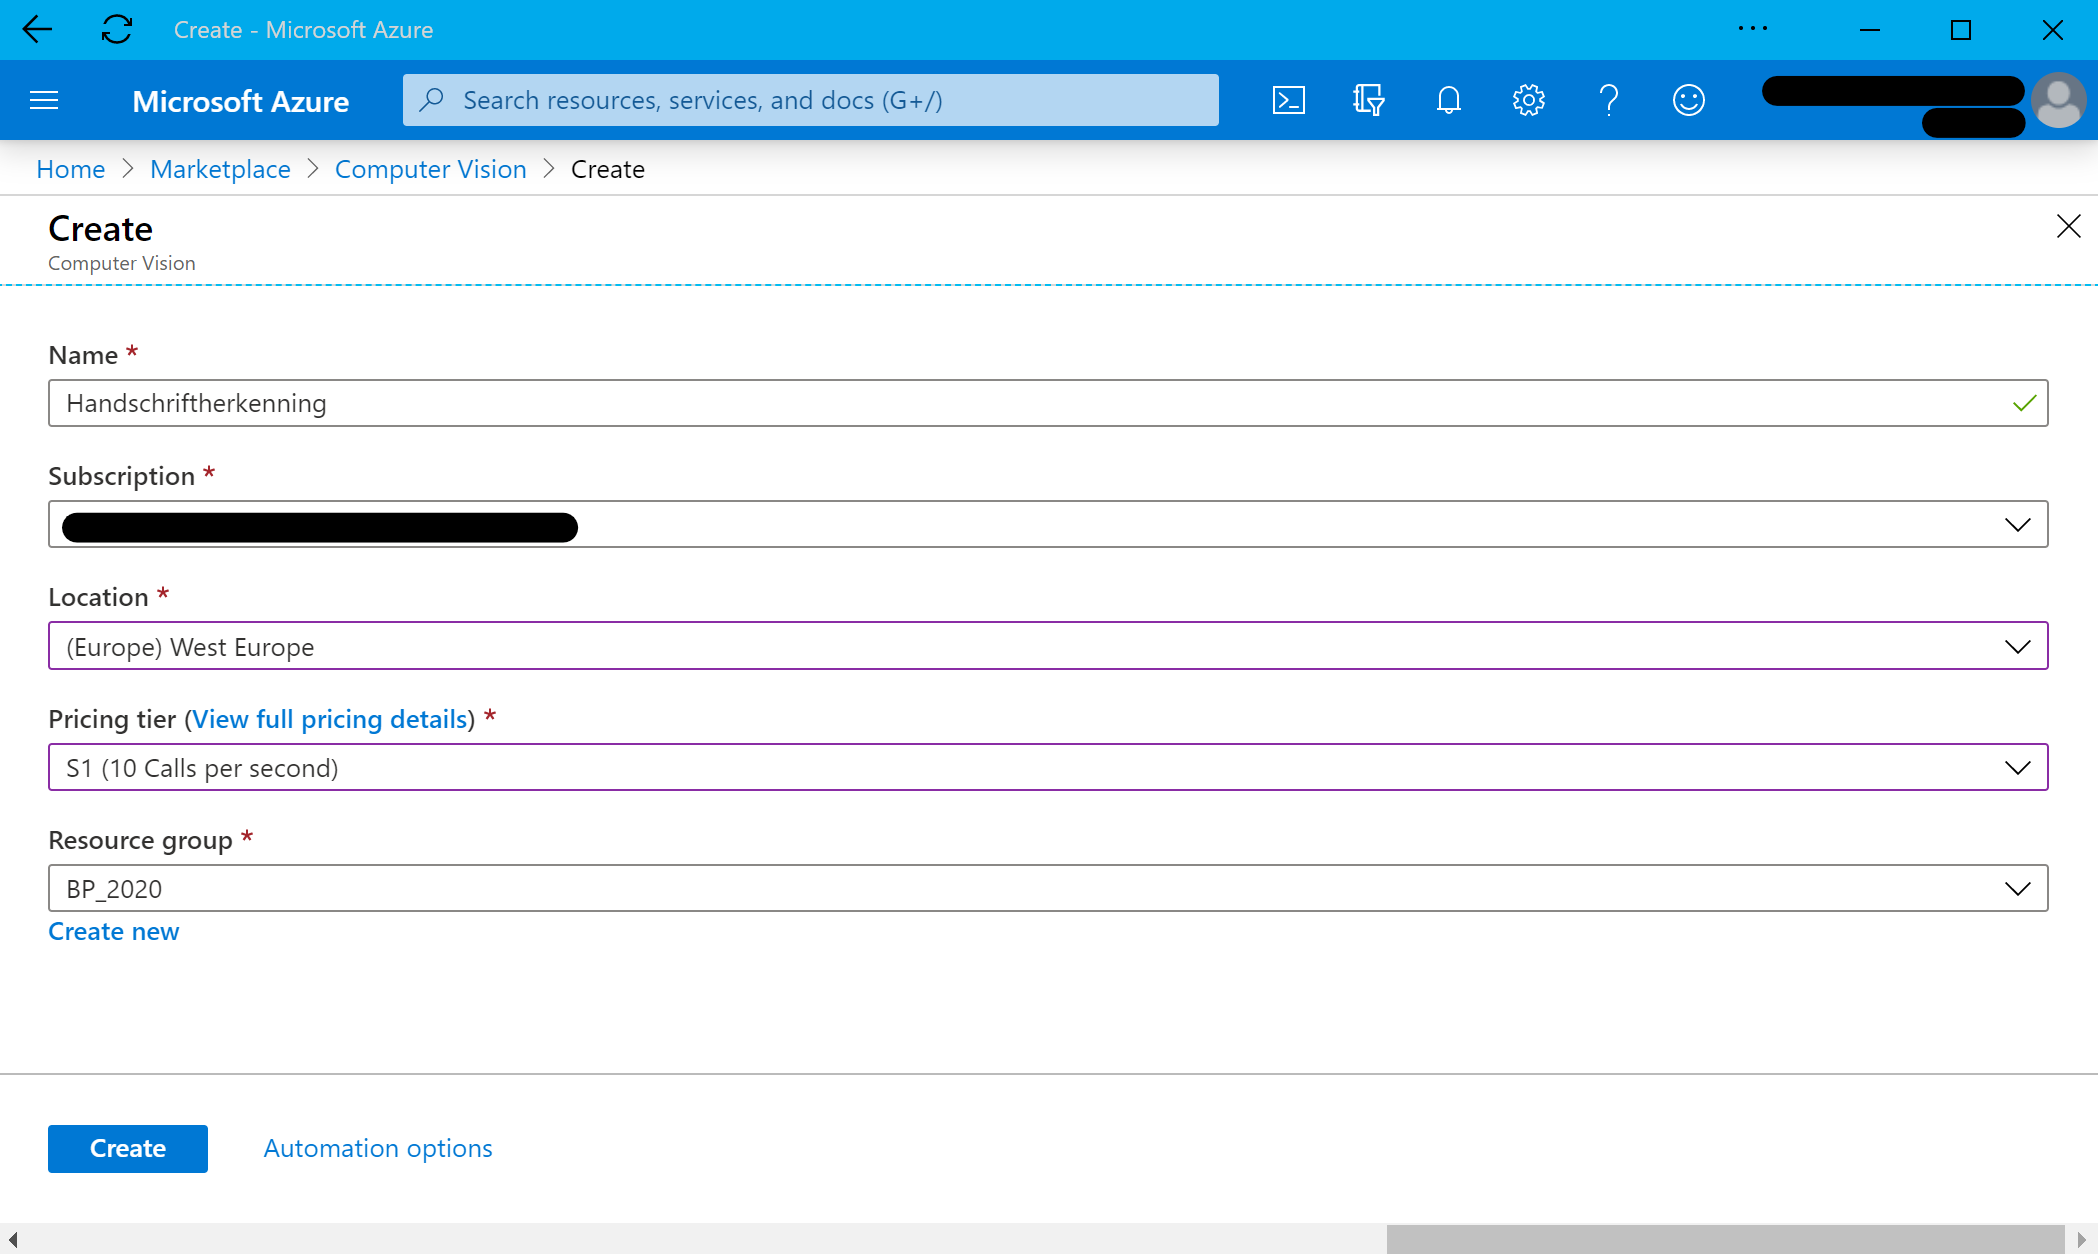
\includegraphics[width=\textwidth,height=\textheight,keepaspectratio]{../../Foto's/computer-vision-config}
	\captionsetup{justification=centering,margin=2cm}
	\caption{Computer Vision creatie pagina. }
	\centering
\end{figure}

De creatie van een Computer Vision instantie verwacht 5 parameters: 

\begin{itemize}
	\item \textbf{Name}
	\item \textbf{Subscription}
	\item \textbf{Location}
	\item \textbf{Pricing tier}
	\item \textbf{Resource group}
\end{itemize}
De naam van een instantie mag enkel bestaan uit alfanumerieke karakters en dient nog niet te bestaan binnen de geselecteerde resource groep. Verder dient de lopende subscriptie van de ingelogde gebruiker geselecteerd te worden. Indien parameters zoals “pricing tier” buiten de scope van de subscriptie gaan krijgt de gebruiker een melding dat de gekozen subscriptie niet volstaat voor de gekozen noden en dat een upgrade nodig is. De gekozen locatie speelt een belangrijke rol als het aankomt op latentie en response time van de API. Hierdoor ligt de beste keuze voor dit onderzoek bij de West-Europese endpoint. 
\newpage
De pricing tier komt in twee verschillende opties:  
\begin{itemize}
	\item \textbf{F0 (20 Calls per minuut)}
	\item \textbf{F1 (10 Calls per seconde)}
\end{itemize}

Beide pricing tiers bieden standaard interactie met de API aan en kan men enkel onderscheiden in het aantal toegelaten transacties per tijdseenheid. De F0 tier volgt een vereenvoudigt transactieplan aangezien dit gratis verkregen kan worden. Bij dit plan wordt er een maandelijkse limiet ingesteld van 5000 transacties samen met een call limiet van 20/minuut. Voor de meeste gebruikers die een niet commerciële actie verrichten, volstaat dit plan. Echter biedt de service ook de S1 tier aan die meer gericht is naar gebruik op Enterprise niveau. Er wordt hierbij voor het Read onderdeel van Computer Vision, een vaste prijs opgesteld van €2.109 per 1,000 transacties. (\cite{Microsoft2020g}) 

\begin{figure}[h]
	
	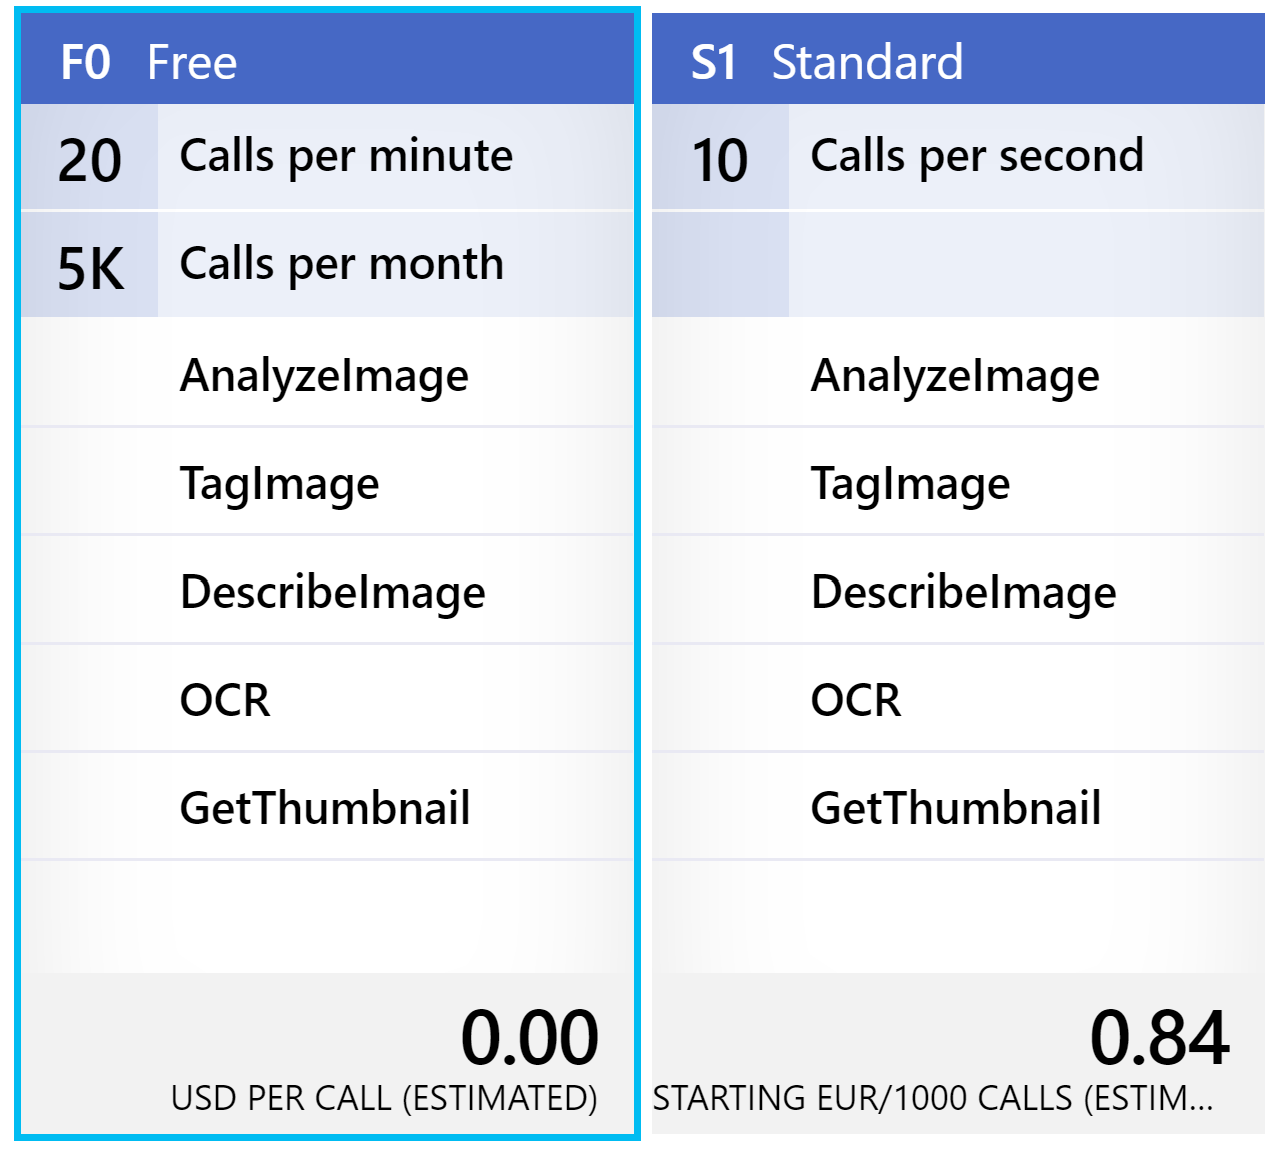
\includegraphics[width=\textwidth,height=\textheight,keepaspectratio]{../../Foto's/computer-vision-pricing}
	\captionsetup{justification=centering,margin=2cm}
	\caption{Pricing tier opties.}
	\centering
\end{figure}
Omdat dit een observatief onderzoek is, volstaat de F0 tier voor het uitvoeren van de test cases en het verzamelen van genoeg data om een conclusie te kunnen trekken. Verdere implementatie van de ontwikkelde software in een productie omgeving kan een hogere tier verwachten. Wanneer men opmerkt dat de F0 tier niet volstaat voor de implementatie, is het mogelijk deze achteraf te upgraden in het API-overzicht (zie fig 4.3). 



Na creatie van de service krijgt men een bevestiging mail toegestuurd met de verwachte uitrol tijd. Dit zou niet langer mogen duren dan 5 minuten. Eens beschikbaar, kan men de onderhoudspagina van de service terugvinden in het Azure dashboard. Hier zijn enkele belangrijke parameters van belang om de nodige communicatie te voorzien met software die calls naar de API verstuurd. Dit zijn namelijk de volgende parameters:  
 
\begin{itemize}
	\item \textbf{API Key }
	\item \textbf{API Endpoint}
\end{itemize}

Elke request uitgevoerd naar de API verwacht een geldige API key en zorgt ervoor dat deze request geautoriseerd wordt (\cite{Microsoft2019a}). Door deze key weet de API ook wat de limieten zijn van het gekozen plan. De API Endpoint is dan de uiteindelijke URL waar de request naar verstuurd wordt. De endpoint bevindt zich dan ook eveneens op de locatie gekozen bij configuratie van de service. De verdere implementatie en het gebruik van deze parameters wordt verder besproken in de volgende sectie.


Het is echter ook nog op te merken dat de huidige versie van de API (Version 3) enkel de extractie van Engels en Spaanse handgeschreven tekst ondersteunt.  Er is in dit onderzoek bewust gekozen om de extractie uit te voeren op Engels geschreven doktersbriefjes. Zoals besproken in hoofdstuk 3, is het verzamelen van handgeschreven teksten in het Nederlands een zeer moeilijke taak. Dit vergt in de meeste gevallen de samenwerking met een tweede partij die willend is om deze data vrij te geven. Daarom is er voor dit onderzoek zoals besproken in hoofdstuk 3, gekozen om gebruik te maken van een Cloud computing model dat getraind is met een generieke dataset. Dit is in zekere zin ook een interessante omgeving waar testen uitgevoerd kunnen worden. Deze testen kunnen aantonen of een generieke dataset even goed presteert bij de extractie van medische termen. In toekomstige versies en naarmate de evolutie van de API, zullen vermoedelijk meerdere talen ondersteunt worden voor extractie, waaronder Nederlands. 

De OCR API ondersteund momenteel wel al de extractie van geprinte tekst in het Nederlands samen met 25 andere talen (\cite{Microsoft2019b}). 


\subsection{Het gebruiken van de API}
De volgende sample code van deze implementatie is beschikbaar op  \href{https://github.com/Helmidyh/HD\_Bachelorscriptie\_Software\_2020}{github},  en werd grotendeels verkregen door \cite{Microsoft2020h} mits enkele aanpassingen voor string parsing. Vervolgens zullen de belangrijkste onderdelen van deze code besproken worden samen met een test request + resultaat. De code werd opgebouwd in C\# .NET en maakt gebruik van het Newtonsoft.Json framework voor eenvoudige interactie en manipulatie van Json bestanden. 
 

\subsection{Authenticatie} 

 

Zoals besproken in de voorgaande sectie, zal elke request verstuurd naar de API, geautoriseerd moeten worden. Dit houdt in dat de API Key meegegeven wordt in de hoofding van de request. Echter is het van enorm belang dat men beide Api Key en Endpoint nooit in code mag terugvinden en dit al zeker niet in een github of productie omgeving. Gebruikers die geen eigenaar zijn van de API kunnen met deze key ongezien requests versturen en data ontvangen. Men kan deze key op enkele manieren verbergen in het project, ook de mogelijkheid is er om gebruik te maken van Azure Keyvault. Hierbij wordt een gezamenlijk overzicht weergeven van al de beschikbare keys van het gebruikers account. Deze zijn achteraf raadpleegbaar met een request call naar de keyvault. 

 

In deze toepassing werd er gekozen om de parameters \textit{subscriptionKey} en \textit{endpoint}, temporeel op te slagen in de  omgevingsvariabelen van het project. Hierdoor worden deze enkel geïnjecteerd bij opstart en zijn ze deels verborgen. 
\newline



\codefragment{java}{parameters.cs}{}
	\textit{Fragment 1.1: Parameters.}


De \textit{uriBase} is een samengestelde parameter bestaande uit de gegenereerde API endpoint van de service, samen met het type request dat men wenst uit te voeren. In dit geval zal de \textit{read} operatie uitgevoerd worden.  

 
\subsection{Opbouwen van een request}
Een read request wordt vervolgens opgebouwd door het initialiseren van een HttpClient. Deze client voegt nodige parameters toe aan de request body en header, vooraleer men deze afvuurt. In fragment 1.2 wordt de API key toegevoegd aan de header. Dit is zoals besproken in sectie 4.0.3 nodig om de request te autoriseren. Verder is het van belang dat de taal van de meegegeven afbeelding gespecifieerd wordt. Momenteel is dit Engels in het formaat “en\_US”, maar in latere stages van de API zal dit evolueren naar Nederlands. 

\newpage
\lstinputlisting{request.cs}
\textit{Fragment 1.2: HttpClient.}




Uiteraard is het van belang dat een afbeelding meegegeven wordt aan de request. Men kan echter niet zomaar een “JPEG” of “PNG” meegeven aan de client. Deze dient eerst omgezet te worden naar een binaire voorstelling van data, in dit geval een array van bytes. Vervolgens wordt deze array van bytes meegegeven aan een instantie van “ByteArrayContent”. Deze instantie combineert de binaire data samen met het “MediaType” van de data. Hierdoor weet de API het type van de meegeleverde data in de body. 
\subsection{Versturen van een request}
Na opzet van de request header en body, kan men de “client” utiliseren om een post request te versturen m.b.v. de methode \textit{PostAsync()} (zie fragment 1.3). Deze methode ontvangt twee parameters, namelijk de “url” en de samengestelde “ByteArrayContent”. Merk op dat deze methode van het type Async is. Dit betekent dat men nooit zeker is wanneer men het beoogde resultaat terugkrijgt van de API en zal dit aldus asynchroon toekomen. 


Om onnodige fouten te vermijden wordt een “await” operator vóór de functie toegevoegd. Deze operator zorgt er voor dat verdere code afhankelijk is van het resultaat van deze response en blokkeert hierbij dus andere threads tót een resultaat verkregen is. 


Het geretourneerde resultaat bevat echter niet de geëxtraheerde tekst, maar één van twee status codes. Bij aanvang van een POST request, zal de API een read operatie uitvoeren op de meegeleverde afbeelding en vervolgens het bekomen resultaat bijhouden. Dit resultaat dient achteraf opgehaald te worden door wijze van een GET request naar de API. In fragment 1.3 wordt een check uitgevoerd op de geretourneerde statuscode. Indien deze van het type “succes” is, bevindt de URI locatie van de geëxtraheerde tekst zich in de header van de response.

\newpage
\lstinputlisting{sendrequest.cs}
\textit{Fragment 1.3: Post request.}


Eens de URI gekend is, wordt deze gebruikt om een GET request op te bouwen. Hierin bevindt zich het uiteindelijke resultaat van de tekst-extractie in JSON formaat. Zoals beschreven in de samplecode van \cite{Microsoft2020h} is de tijd van teruggave afhankelijk van de hoeveelheid te verwerken tekst. Daarom wordt aangetoond in fragment 1.4, dat om de 1000 ms een check gedaan wordt op de beschikbaarheid van de data. 




\lstinputlisting{sendrequest.cs}
\textit{Fragment 1.4: Get request.}

\subsection{Response}
Dit concludeert in grote lijnen de werking van de API, in de volgende sectie wordt een eenvoudige test request opgezet met een beter inzicht op wat voor data de API precies retourneert en hoe deze gebruikt kan worden in een probleem dat zich kan voordoen in de echte wereld. In eerste instantie zal dit een JSON-string zijn met een aantal zeer specifieke eigenschappen van elk gedetecteerd woord. 

Om dusdanig de software te gaan testen, wordt op figuur 4.4 gebruik gemaakt van een redelijk leesbaar doktersbriefje. Merk op dat deze voorschriften drastisch kunnen variëren en dat deze verschillende vormen kunnen aannemen.  
\begin{figure}
	\newpage
	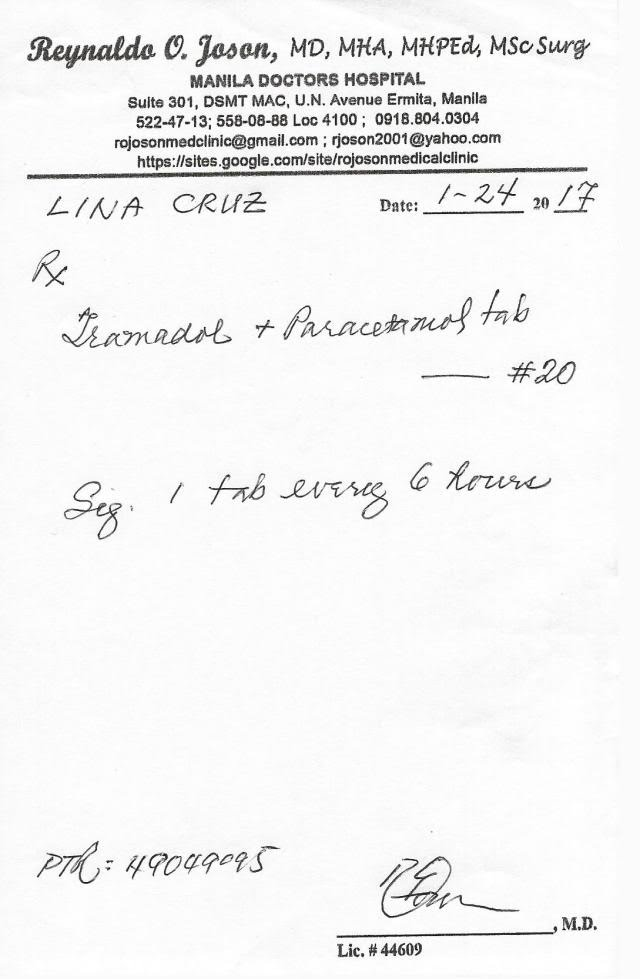
\includegraphics[width=\textwidth,height=\textheight,keepaspectratio]{../../Foto's/prescription_legible_roj_17jan24}
	\captionsetup{justification=centering,margin=2cm}
	\caption{Doktersbriefje voorbeeld. \cite{Joson2017}}
	\centering
\end{figure}


Een eerste uitdaging is dus om na te gaan of medische termen, meer bepaald medicatie zoals “Tramadol” en “Paracetamol” gezien in figuur 4.4, gedetecteerd worden. Dit zou enerzijds al een eerste stap zijn om een conclusie te trekken bij dit onderzoek. De volledige handgeschreven tekst die als persoon waargenomen wordt zou dus het volgende zijn:

\begin{itemize}
\item LINA CRUZ 
\item PX
\item Tramadol + Paracetamol tab 
\item  \#20 
\item Seg. 1 tab every 6 hours 
\item PTR : 49049095 
\end{itemize}

Vervolgens laten we de software los op figuur 4.4 en bekijken de uitkomst. Het ruwe JSON-resultaat is terug te vinden op \href{https://github.com/Helmidyh/HD\_Bachelorscriptie\_Software\_2020}{github} maar zal voor leesbaarheid geparsed worden naar een duidelijker resultaat. \cite{Microsoft2017} beschrijft de parameters in deze geretourneerde JSON als volgt: 

\begin{itemize}
\setlength\itemsep{1em}
\item \textbf{Status:} De teruggekeerde status van de request,  mogelijks “succeeded”, "notStarted", "failed" en "running". Vanaf deze status op "succeeded" komt te staan, zal het JSON-bestand de herkende tekst bevatten.  

\item \textbf{Lines:} Een lijst van herkende zinnen. Het maximum aantal lijnen dat op één pagina gedetecteerd kan worden is 300. Hierbij worden deze lijnen gesorteerd op de volgorde waarin deze gedetecteerd werden (van linksboven naar rechtsonder). De lijnen stellen dan in de meeste gevallen ook een volledige zin voor. 

\item \textbf{Text:} Een volledig herkende zin in één lijn, deze wordt verder opgesplitst in een lijst van woorden.

\item \textbf{Words:} Een verzameling van woorden in een herkende zin.

\item \textbf{BoundingBox:} Een rechthoek dat de positie bevat van de herkende zin of het herkende woord, gespecifieerd als een lijst bestaande uit 8 nummers. Deze nummers stellen de coördinaten van het herkende woord voor, relatief aan de linkerbovenhoek van de afbeelding. Dit zijn dus 4 paren van x,y coördinaten waardoor een rechthoek gevormd wordt (zie fragment 1.5). 

\item \textbf{Confidence:} Het vertrouwensniveau van elk gedetecteerd woord. Zoals beschreven in hoofdstuk 2, zou dit voor handgeschreven teksten lager moeten liggen dan getypte tekst. 
\end{itemize}

\newpage
Om in het volgende hoofdstuk collectief de resultaten op een eenvoudige wijze te vergelijken en samen te vatten, wordt dus gebruik gemaakt van een parsing methode. Deze methode genereerd een overzicht dat enkel de zin, de woorden en het vertrouwensniveau weergeeft, wat uiteraard ook de belangrijkste attributen zijn. 



In fragment 1.5 wordt een deel van het ruwe geretourneerde resultaat weergeven. Merk op dat voor de leesbaarheid, de “boundingBox” parameter van elk specifiek woord weggelaten is, aangezien men een algemene “boundingBox” van de volledige zin ter beschikking heeft. 

\lstinputlisting{rawresult.json}
\textit{Fragment 1.5: Ruw resultaat.}
\newpage
\lstinputlisting{parsedresult.txt}
\textit{Fragment 1.6: Parsed resultaat.}


Men kan duidelijk zien dat mits de lage vertrouwenswaarde, de zin “Tramadol + Paracetamol tab” volledig juist geëxtraheerd is. Dit resultaat stelt wel degelijk voor dat medische termen opgenomen zijn bij het trainen van het extractie model. Verder worden de rest van de handgeschreven zinnen vlekkeloos overgenomen. Dit toont enerzijds aan hoe accuraat dit model is mits dit nog een zeer recente technologie is.  


Als de gemiddelde accuraatheid genomen wordt van elk woord, denkt de API de tekst met een accuraatheid van 59\% voorspeld te hebben. In principe ligt dit percentage relatief laag aangezien men kan vaststellen dat de meerderheid van de woorden volledig juist voorspeld werden. Verder, was de responsetijd van de API was in dit geval +- 8.673 seconden. 

\subsection{Conclusie}
Uit dit hoofdstuk kunnen we concluderen dat het wel degelijk mogelijk is om handschrift te extraheren van een afbeelding. Dit enerzijds rekening houdend met medische termen en opschriften.  Wat nu momenteel echter in vraag gesteld wordt, is of dit resultaat aanhoudend is. Hoe reageert de API tegenover een ander type doktersbriefje, schrijfstijl of kleur? Het is onmogelijk om duizenden testen op te zetten om elke specifieke karakteristiek dat in een doktersbriefje kan voorkomen, te testen. 

In het volgende hoofdstuk worden enkele van deze algemeen gerichte vragen in een test gegoten. 
\chapter{Test cases}

Uit het vorige hoofdstuk kon men vaststellen dat de Computer Vision API wel degelijk een bruikbaar resultaat levert. Dit resultaat kan verder gemanipuleerd worden voor verscheidene use cases die zich kunnen voordoen in eender welk domein. In figuur 3.4 van hoofdstuk 4 werd een semi leesbaar doktersbriefje gebruikt. In principe was dit een perfect voorbeeld om enkel de functionaliteit van de API te testen. Echter is het van belang om na te gaan waar de API de lijn trekt.  



Om die redenen werden er in het volgende hoofdstuk drie test cases opgesteld. Elke van deze test cases bestaat uit één of meerdere doktersbriefjes. Hierbij werden deze voorgesteld aan aantal personen om na te gaan hoe zij deze tekst interpreteerden. Achteraf werd van elk geïnterpreteerd woord de populairste interpretatie genomen en vergeleken met het resultaat van de API.  

Hierdoor is het mogelijk om een rechtstreekse vergelijking uit te voeren van hoe mensen een onleesbare tekst interpreteren vergeleken met een AI-toepassing. 

Eveneens wordt er per extractie een tabel opgesteld met het geëxtraheerde woord, de interpretatie en de herkenningsgraad. 
\newpage
\section{Test Case 1}
\subsection{Opzet}
De eerste test case zal nagaan wat het effect van een verlaagde resolutie is op de extractie. Om dit effectief te gaan testen zal men gebruik maken van hetzelfde doktersbriefje in figuur 4.4 

Echter werd een kwaliteitscompressie op deze afbeelding uitgevoerd waarbij deze nog maar 60 \% van de originele kwaliteit bevat (zie fig 5.2). Vooraleer een vergelijking kan plaatsvinden, werd een statistische tabel van de originele extractie request opgesteld in figuur 5.1. Men kan duidelijk vaststellen dat de meerderheid van de woorden correct voorspeld werden.  

\begin{figure}[h]
	
	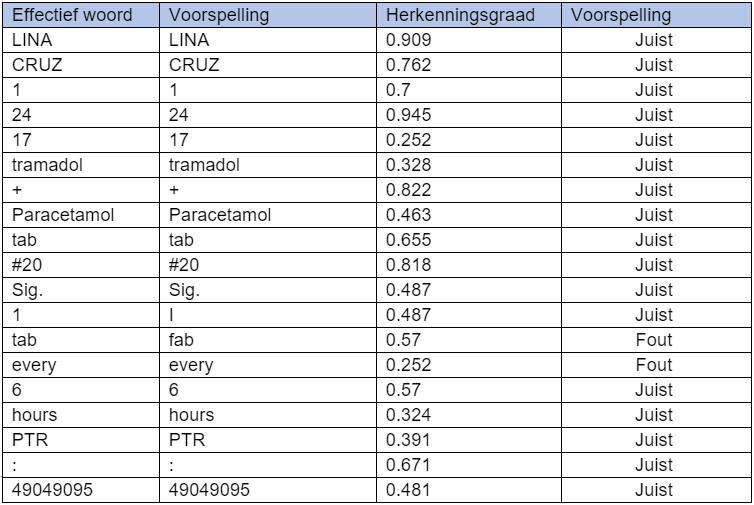
\includegraphics[width=\textwidth,height=\textheight,keepaspectratio]{../Foto's/doktersbriefje0_tabel}
	\captionsetup{justification=centering,margin=2cm}
	\caption{Doktersbriefje voorbeeld statistiek  100\% kwaliteit. \cite{}}
	\centering
\end{figure}
\subsection{Doktersbriefje verlaagde kwaliteit resultaat}
Wanneer naar figuur 5.2 gekeken wordt, ziet men op het eerste zicht visueel geen grote verschillen in kwaliteit, echter kan dit wel een invloed hebben op de extractie kwaliteit. Meer bepaald de virtuele “ruis”. Deze ruis kan karakters vervormen en in extreme gevallen deze zelfs onherkenbaar maken. Vervolgens werd er een extractie request afgevuurd op figuur 5.2 en werd de verkregen data hiervan in tabel 5.3 weergegeven.
\begin{figure}[h]
	
	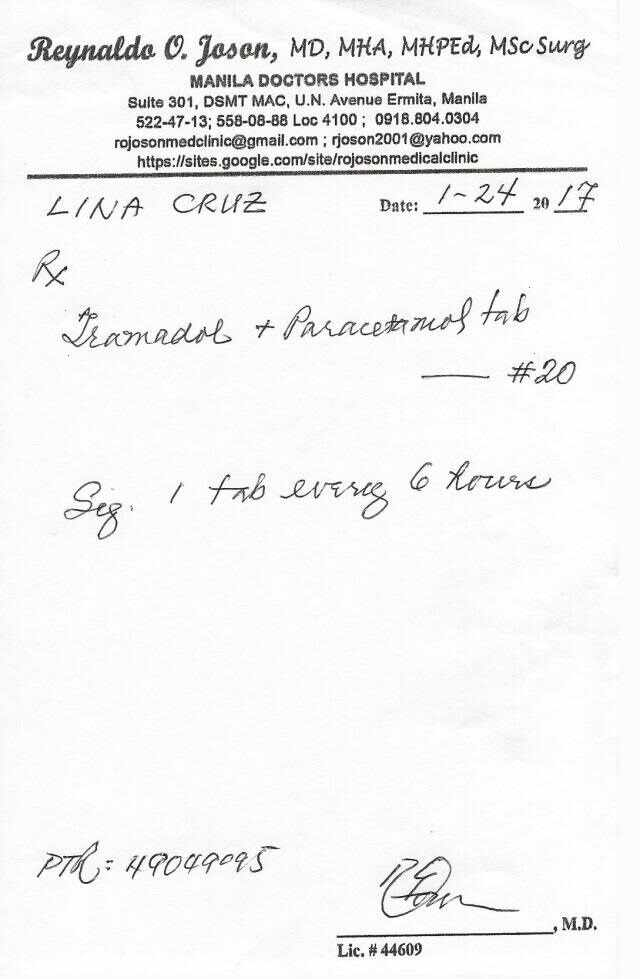
\includegraphics[width=\textwidth,height=\textheight,keepaspectratio]{../doktersbriefjes/61procent}	
	\captionsetup{justification=centering,margin=2cm}
	\caption{Doktersbriefje voorbeeld 60\% kwaliteit. \cite{}}
	\centering
\end{figure} 

\clearpage
\begin{figure}[h]
	
	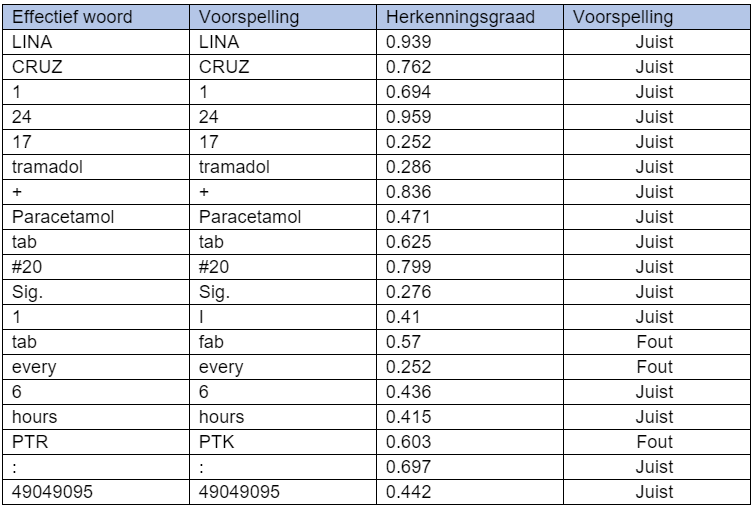
\includegraphics[width=\textwidth,height=\textheight,keepaspectratio]{../Foto's/doktersbriefje0_60procent_tabel}
	\captionsetup{justification=centering,margin=2cm}
	\caption{Doktersbriefje voorbeeld statistiek 100\% kwaliteit. \cite{}}
	\centering
\end{figure}


Wanneer men beide tabellen vergelijkt zijn er enkele verschillen die meteen naar voor komen. Zoals verwacht is de algemene herkenningsgraad gedaald. De meerderheid van de woorden werden nog steeds juist voorspeld echter met een lagere herkenningsgraad. Er werd één woord vergeleken met figuur 4.4 verkeerd voorspeld, namelijk "PTR". Dit stelt voor dat een lagere resolutie wel degelijk invloed kan hebben op de extractie. Narmate de verlaging in kwaliteit zullen meer en meer woorden verkeerd voorspeld worden.



\section{Test Case 2}
\subsection{Opzet}
De tweede test case is een meer generiek gerichte test, hierbij wordt gekeken naar de algemene accuraatheid van de teruggegeven data en het aantal juiste voorspellingen. Hier werd een andere aanpak genomen tegenover test case 1. De juistheid wordt hierbij bepaald door de voorspelling te vergelijken met een interpretatie. Hierbij werden vier doktersbriefjes voorgesteld aan een groep mensen. Elke persoon in deze groep probeerde de handgeschreven tekst in deze doktersbriefjes zo accuraat mogelijk te interpreteren.  Achteraf werd de gemiddeld populairste interpretatie van elk woord genomen en in een tabel gegoten. Door een vergelijking uit te voeren van het voorspelde met de interpretatie, kan men nagaan of de API handgeschreven woorden op dezelfde manier interpreteert als mensen. 
%%=============================================================================
\subsection{Doktersbriefje 1 resultaat}
Zoals men kan zien op figuur 5.4 zijn er in totaal 23 woorden/karakters geëxtraheerd. Hierbij zijn 14 van deze 25 correct voorspeld naargelang de interpretatie. Merk op dat men de interpretatie niet als volledig betrouwbaar mag beschouwen. Een persoon kan zonder medische achtergrond of kennis een woord op een volledig andere manier interpreteren dan iemand die ervaring heeft in dit domein. Een voorbeeld hiervan zijn de woorden “amoxicillin” en “Himox”, de populairste interpretatie hiervan werd gezien als “omoxirillin” en “Hinlox”.  


Echter kan men deze voorspelling niet zoals in andere gevallen fout beschouwen, want “amoxicillin” en “Himox” zijn medisch correcte termen. Men kan dus wel degelijk vaststellen dat medische termen in hun geheel correct voorspeld kunnen worden, echter is hier wel nog een manuele controle voor nodig.  In conclusie kan men een gemiddelde herkenningsgraad van 0.45087 per woord vinden, met 60\% van deze woorden correct voorspeld. 
\begin{figure}[h]
	
	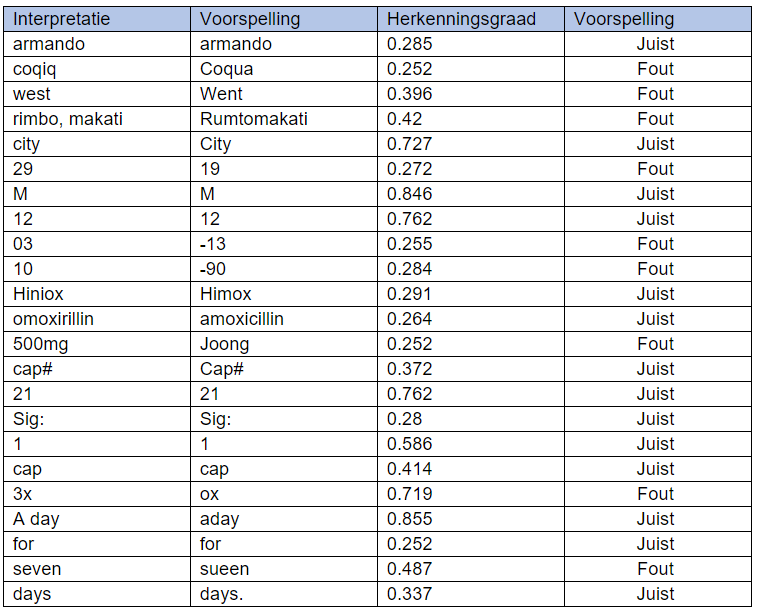
\includegraphics[width=\textwidth,height=\textheight,keepaspectratio]{../Foto's/doktersbriefje1_tabel}
	\captionsetup{justification=centering,margin=2cm}
	\caption{Doktersbriefje 1 extractie resultaat}
	\centering
\end{figure}
\clearpage
\begin{figure}
	
	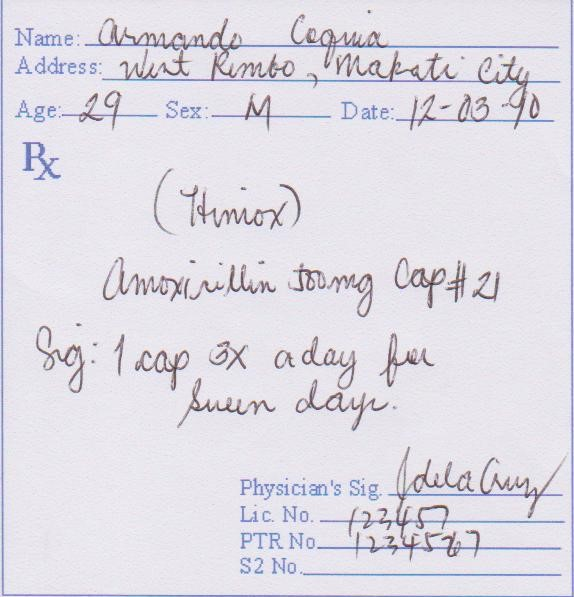
\includegraphics[width=\textwidth,height=\textheight,keepaspectratio]{../doktersbriefjes/dokterbriefje_1.jpg}
	\captionsetup{justification=centering,margin=2cm}
	\caption{Doktersbriefje 1. (\cite{Tacio2013})}
	\centering
\end{figure}
\clearpage
%%=============================================================================

%%=============================================================================
\subsection{Doktersbriefje 2 resultaat}
Bij de resultaten van de extractie op figuur 5.7 zijn er in totaal 22 woorden geëxtraheerd, waarvan 2 onbepaald. Eveneens zijn bij de interpretatie 3 woorden als onbepaald verklaard. Dit fenomeen doet zich voor wanneer bepaalde woorden onherkenbaar zijn voor de API, waardoor deze overgeslagen worden. Dit was dus het geval bij de interpretatie van “biovik 100 mg tab”. 


Een mogelijke oorzaak kan zijn dat 2 woorden te dicht bij elkaar staan of dat de gebruikte inkt mogelijks te licht is. Verder werden bepaalde woorden simpelweg oninterpreteerbaar verklaard door de testgroep, waardoor deze niet zullen bijdragen tot het gehele resultaat. De gemiddelde herkenningsgraad mits onbepaalde woorden is 0.525182, met 58 \% van de voorspelde en geïnterpreteerde woorden correct voorspeld. 
\begin{figure}[h]
	
	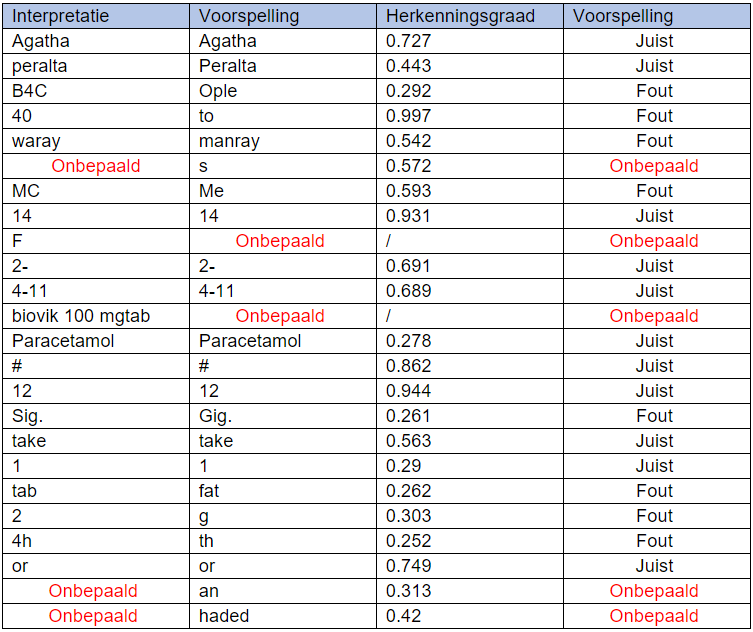
\includegraphics[width=\textwidth,height=\textheight,keepaspectratio]{../Foto's/doktersbriefje2_tabel}
	\captionsetup{justification=centering,margin=2cm}
	\caption{Doktersbriefje 2 extractie resultaat}
	\centering
\end{figure}
\clearpage
\begin{figure}
	
	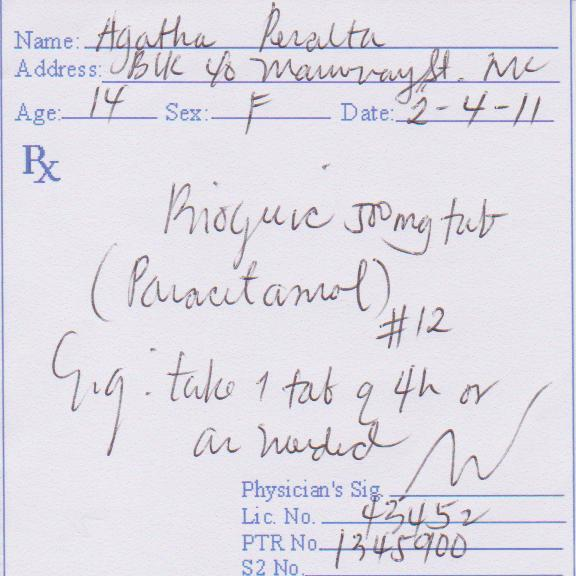
\includegraphics[width=\textwidth,height=\textheight,keepaspectratio]{../doktersbriefjes/dokterbriefje_2.jpg}
	\captionsetup{justification=centering,margin=2cm}
	\caption{Doktersbriefje 2. (\cite{Tacio2013})}
	\centering
\end{figure}
\clearpage
%%=============================================================================

%%=============================================================================
\subsection{Doktersbriefje 3 resultaat}
Volgens de resultaten van de extractie op figuur 5.9 zijn er in totaal 21 woorden geëxtraheerd, waarvan 1 onbepaald. Tegenover extractieresultaat 5.6 zijn hier veel minder woorden als onbepaald verklaard. Dit lijkt in zeker zin ook logisch als men kijkt naar de algemene slordigheid van figuur 5.7 vergeleken met figuur 5.9 Een terugkerende trend die men kan waarnemen bij deze resultaten, is de voorspelling van de medicatie dosering.  

Deze is in geen enkel van de gevallen tot nu toe juist voorspeld. De gemiddelde herkenningsgraad mits 1 onbepaald woord is 0.507048 met 57 \% van de voorspelde en geïnterpreteerde woorden correct voorspeld. 
\begin{figure}[h]
	
	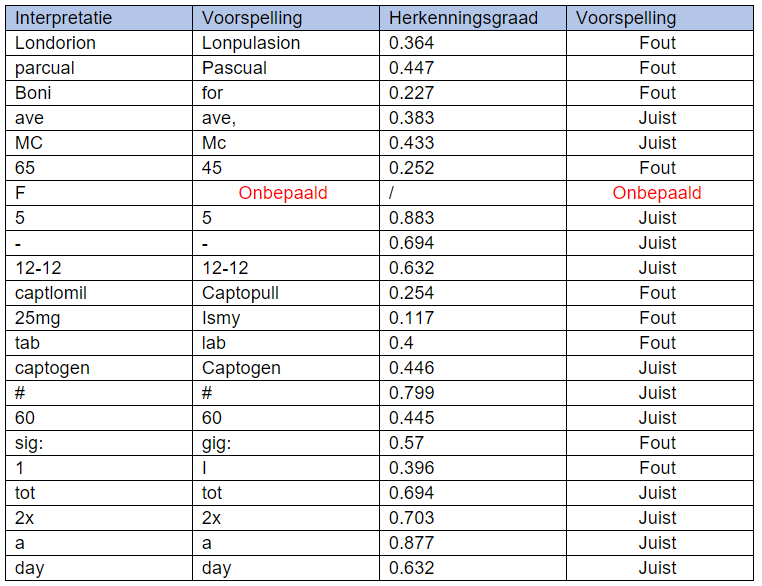
\includegraphics[width=\textwidth,height=\textheight,keepaspectratio]{../Foto's/doktersbriefje3_tabel}
	\captionsetup{justification=centering,margin=2cm}
	\caption{Doktersbriefje 3 extractie resultaat}
	\centering
\end{figure}
\clearpage
\begin{figure}
	
	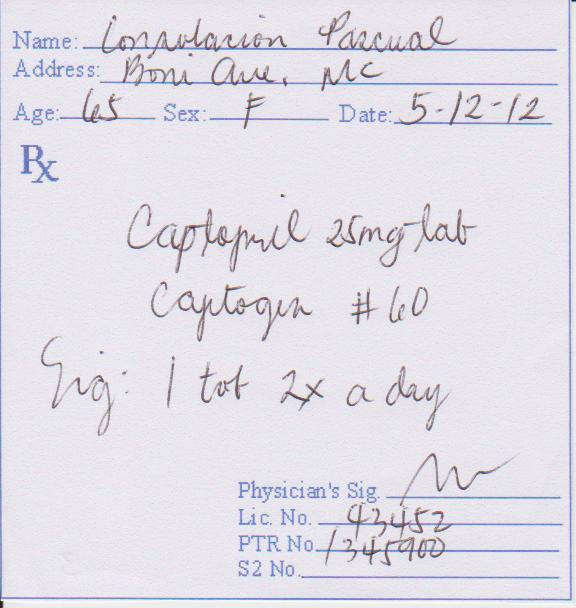
\includegraphics[width=\textwidth,height=\textheight,keepaspectratio]{../doktersbriefjes/dokterbriefje_3.jpg}
		\captionsetup{justification=centering,margin=2cm}
	\caption{Doktersbriefje 3. (\cite{Tacio2013})}
	\centering
\end{figure}
\clearpage
%%=============================================================================

%%=============================================================================
\subsection{Doktersbriefje 4 resultaat}
Bij de laatste extractie request ziet men positieve resultaten. Hierbij zijn 27 woorden geëxtraheerd, zonder onbepaalde voorspellingen. Merk op dat de meerderheid van de foutief gerekende voorspellingen, maar 1 karakter verschillen van de interpretatie. 


Een toekomstige oplossing voor dit probleem zou een fuzzy matching NLP model kunnen zijn. Hierbij worden woorden die enkele karakters van het originele afwijken, vergeleken met een generieke databank. Men kan op deze manier woorden die niet volledig juist verklaard zijn toch nog goedkeuren door wijze van vergelijking. Echter zou dit uiteraard de kost en tijd van extractie enkel maar vergroten. Kijkend naar het resultaat, werd er een gemiddelde herkenningsgraad van 0.564259 per woord bekomen, waarbij  64\% van de interpretatie correct voorspeld. 
\begin{figure}[h]
	
	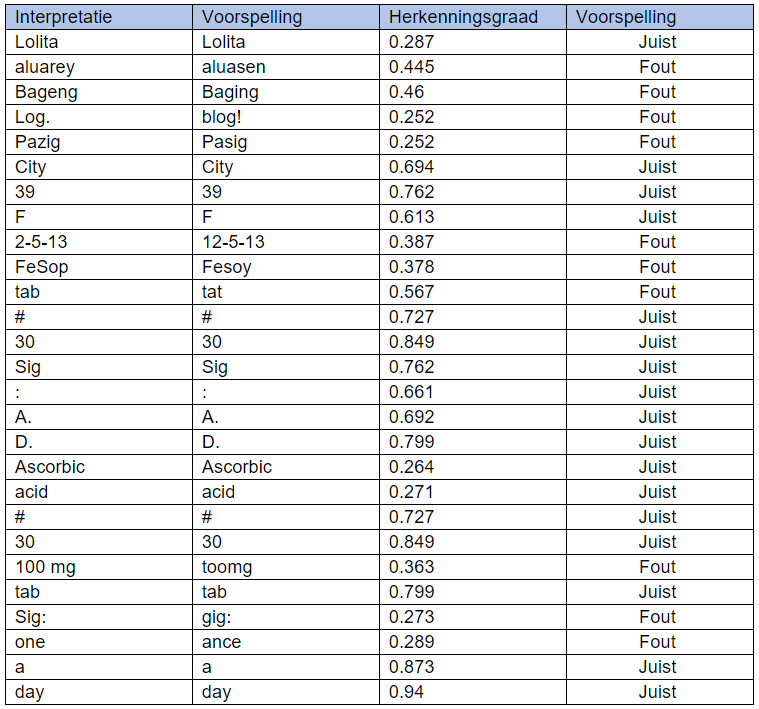
\includegraphics[width=\textwidth,height=\textheight,keepaspectratio]{../Foto's/doktersbriefje4_tabel}
	\captionsetup{justification=centering,margin=2cm}
	\caption{Doktersbriefje 4 extractie resultaat}
	\centering
\end{figure}
\clearpage
\begin{figure}
	
	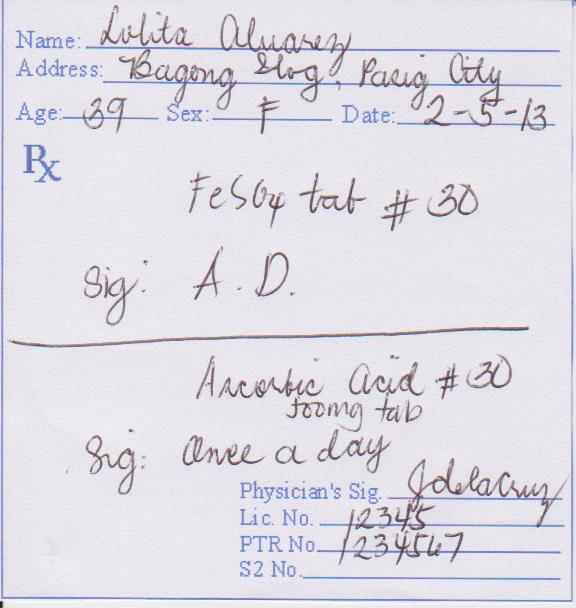
\includegraphics[width=\textwidth,height=\textheight,keepaspectratio]{../doktersbriefjes/dokterbriefje_4.jpg}
	\captionsetup{justification=centering,margin=2cm}
	\caption{Doktersbriefje 4. (\cite{Tacio2013})}
	\centering
\end{figure}
\clearpage
%%=============================================================================

\section{Test Case 3}
\subsection{Opzet}
De derde en laatste test case zal nagaan of het uiterlijk van een doktersbriefje invloed heeft op het gemiddelde resultaat. Voorgaande doktersbriefjes gebruikt in test case 2, maakten gebruik van éénzelfde template. Men bekomt hierdoor een gestroomlijnd resultaat waarbij men de uitkomst enkel kan baseren op het handgeschrift. Echter is het wel nog interessant om een extractie uit te voeren op een doktersbriefje dat gebruik maakt van een ander template. Hierbij wordt de positionering en volgorde van extractie mogelijks anders opgenomen door de API. 
Bij deze test werd gebruik gemaakt van het doktersbriefje weergeven in figuur 5.13. Merk op dat meerdere karakteristieken van figuur 5.13 duiden op een suboptimale extractie. Hierbij ziet men net zoals in test case 1, een lage resolutie gepaard met een slordig handschrift. In essentie stelt deze test een extreem geval voor dat zelden zal voorkomen bij een echte implementatie. 

\subsection{Doktersbriefje 5 resultaat}
Kijkend naar de resulterende data zichtbaar of figuur 5.12, kan men vaststellen dat de gemiddelde herkenningsgraad 0.496833 bedraagt. In totaal werd 50 \% van de interpretaties correct voorspeld door de API. Dit wijst m.a.w. op een daling van +- 8 \% tegenover de voorgaande resultaten. De meerderheid van de medische termen zijn hierbij wel correct voorspeld, met de tot nu toe enige correcte voorspelling van de medische dosering. 
\begin{figure}[h]
	
	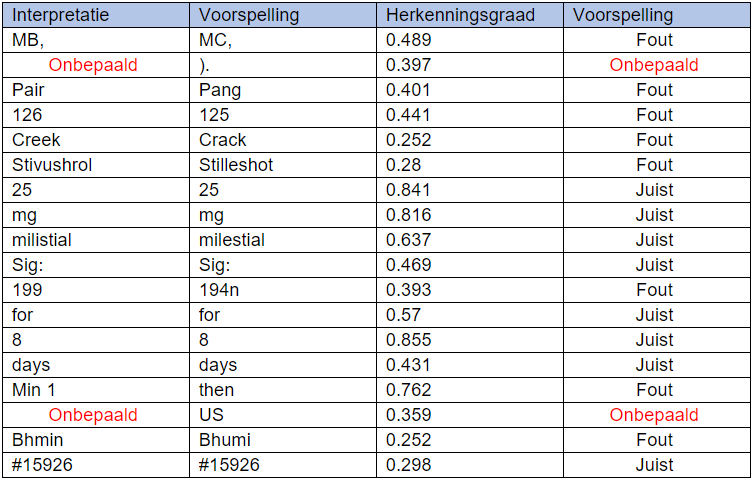
\includegraphics[width=\textwidth,height=\textheight,keepaspectratio]{../Foto's/doktersbriefje5_tabel}
		\captionsetup{justification=centering,margin=2cm}
	\caption{Doktersbriefje 5 extractie resultaat}
	\centering
\end{figure}
\clearpage
\begin{figure}
	
	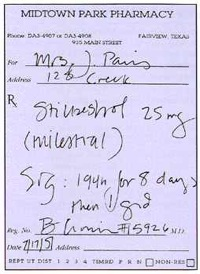
\includegraphics[width=\textwidth,height=\textheight,keepaspectratio]{../doktersbriefjes/dokterbriefje_5.jpg}
		\captionsetup{justification=centering,margin=2cm}
	\caption{Doktersbriefje 5. (\cite{Abrahams2008})}
	\centering
\end{figure}
\clearpage
\section{Resultaten}
Na het uitvoeren van de tests, kunnen we collectief de resultaten verzamelen en vergelijken.  
\subsection{Test cases}
Op figuur 5.14 ziet men een weergave van de bekomen extractie percentages.  Kijkend naar test 1, werd 84 \% van de geëxtraheerde woorden correct voorspeld. Vergeleken met de percentages bekomen in test case 2 en 3, ligt dit relatief hoog. Een mogelijke verklaring voor dit hoge percentage zou kunnen liggen bij de ruimere spreiding van de woorden op figuur 5.2.  



Extracties 2-5 uitgevoerd in test case 2, tonen een relatief gelijkaardig resultaat. Bij deze test case werden 4 doktersbriefjes met éénzelfde template getest. Gemiddeld werd 59.75 \% van de woorden correct voorspeld. De meerderheid van de foutieve voorspellingen lag bij de naam of het adres van de persoon in kwestie. In principe was dit te verwachten aangezien de focus bij de dataset minder ligt op unieke naamgevingen. Wat men echter wel kan vaststellen is dat de meerderheid van de medische termen correct voorspeld werden, wat bijdrage levert aan een positief resultaat. 



Test case 3 toonde, vergelijkend met test case 2, relatief weinig tot geen verschil aan in resultaat. Dit geeft enerzijds ook aan dat het uiterlijk van een doktersbriefje het resultaat niet ongewild beïnvloedt. Wat echter wel een tegenargument voor deze bewering kan zijn is dat de spreiding van de woorden, gezien bij doktersbriefje 1, bekomen werd door een groter schrijfvlak. Wat op zijn beurt weer een beter resultaat zou geven. 




 

\begin{figure}[h]
	
	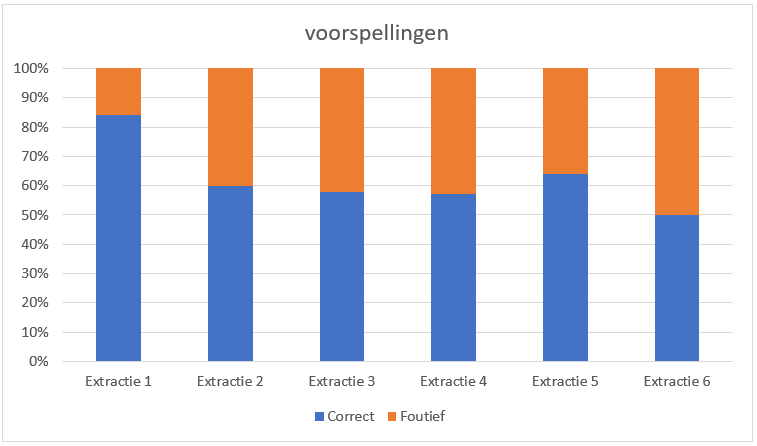
\includegraphics[width=\textwidth,height=\textheight,keepaspectratio]{../Foto's/voorspellingen_statistiek.png}
		\captionsetup{justification=centering,margin=2cm}
	\caption{Statestiek voorspellingen.}
	\centering
\end{figure}
 \clearpage
\subsection{Herkenningsgraad}
Verder, werd in figuur 5.15 het verloop van de herkenningsgraad per geëxtraheerd woord weergeven. Elke weergeven lijn stelt de volgorde voor waarin elk woord voorspeld werd, waarbij de y-as de zekerheid van extractie in \% voorstelt. Zoals eerder beschreven, ligt de meerderheid van foutieve voorspellingen bij de extractie van naam of adres. De oorzaak hiervan zou enerzijds liggen bij gebrek aan opname van unieke naamgevingen bij de training van het model. 


Merk op dat men dit fenomeen duidelijk kan waarnemen in figuur 5.15. De naam en adres van de patiënt worden in de meeste gevallen en dus ook bij de gebruikte doktersbriefjes bovenaan weergeven. Aangezien in hoofdstuk 4 (sectie 4.0.6) beschreven werd dat de API, een lijn extractie van linksboven naar rechtsonder uitvoert, zullen deze dus eerst geëxtraheerd worden. Men ziet ook wel degelijk dat de eerste 4-5 woorden bij elke extractie zelden een herkenningsgraad boven de 50 \% hebben.


\begin{figure}[h]
	
	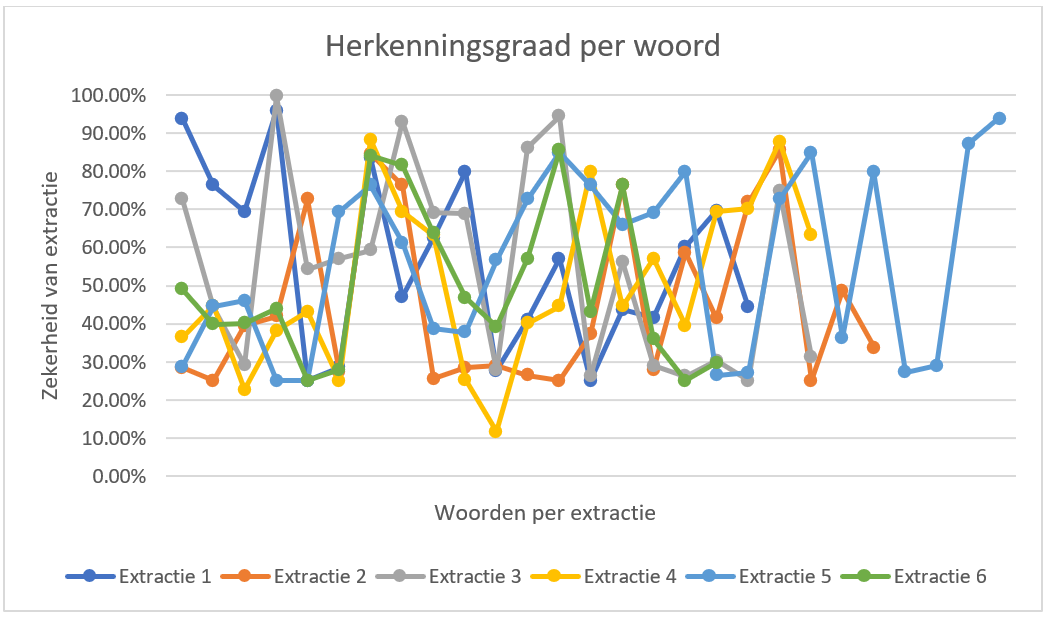
\includegraphics[width=\textwidth,height=\textheight,keepaspectratio]{../Foto's/herkenningsgraad_statistiek.png}
		\captionsetup{justification=centering,margin=2cm}
	\caption{Verloop van de herkenningsgraad per extractie.}
	\centering
\end{figure}

Collectief was de API bij het uitvoeren van de 3 test cases, per woord, gemiddeld 52 \% zeker van zijn voorspelling. Dit getal zal uiteraard evolueren, naargelang het aantal testen dat men uitvoert, vergroot en de variatie van het type doktersbriefjes toeneemt. 
\newpage
\section{Conclusie}
Uit de resultaten kon men vaststellen dat de Computer Vision API wel degelijk bruikbaar is voor het extraheren van doktersgeschrift. Hierbij werd de meerderheid van de woorden correct voorspeld, gepaard met de juiste medische termen. De interpretaties verzameld door de testgroep werden grotendeels ook door de API voorspeld. Het is echter wel op te merken dat bij deze tests maar een beperkt aantal doktersbriefjes gebruikt werd. Dit komt grotendeels door de beperkte beschikbaarheid en vrijstelling van dit type document. Uiteraard zijn de meeste mensen niet bereid om hun naam en gegevens open te stellen aan een breder publiek. Aangezien het bekomen van test cases al een moeilijke zaak was zou dit al zeker een hindernis vormen bij het trainen van een volledig extractie model. 


De Computer Vision service die bij dit onderzoek gebruikt werd, kan maximaal 5000 requests per maand ontvangen. Deze oplossing is ruim schaalbaar door middel van de Azure Cloud en kan mogelijks met enige configuratie op een eenvoudige wijze in een productie omgeving tewerkgesteld worden, mits hier een bruikbaar plan voor gekozen is. 


Collectief kon men vaststellen dat de API gemiddeld 62\% van een doktersbriefje volledig juist kan voorspellen. Wanneer de ontwikkelde software gebruikt zou worden in een productie omgeving waar eenzelfde type briefje voorkomt, dan zou men een meer gestroomlijnd resultaat bekomen. 


Uiteraard is het onmogelijk om enkel uit deze uitgevoerde testen een volledige conclusie te trekken, maar het wijst wel degelijk richting een positief resultaat. 








% Voeg hier je eigen hoofdstukken toe die de ``corpus'' van je bachelorproef
% vormen. De structuur en titels hangen af van je eigen onderzoek. Je kan bv.
% elke fase in je onderzoek in een apart hoofdstuk bespreken.

%\input{...}
%\input{...}
%...

%%=============================================================================
%% Conclusie
%%=============================================================================

\chapter{Conclusie}
\label{ch:conclusie}

% TODO: Trek een duidelijke conclusie, in de vorm van een antwoord op de
% onderzoeksvra(a)g(en). Wat was jouw bijdrage aan het onderzoeksdomein en
% hoe biedt dit meerwaarde aan het vakgebied/doelgroep? 
% Reflecteer kritisch over het resultaat. In Engelse teksten wordt deze sectie
% ``Discussion'' genoemd. Had je deze uitkomst verwacht? Zijn er zaken die nog
% niet duidelijk zijn?
% Heeft het onderzoek geleid tot nieuwe vragen die uitnodigen tot verder 
%onderzoek?
Bij aanvang van deze studie werden de limitaties van handschriftherkenning op de proef gesteld. Hiermee kwam de CM initieel met de vraag of dergelijke software instaat was om handgeschreven teksten van een doktersbriefje te extraheren. Uit de voorgaande literatuurstudie bleek dat Cloud Computing de laatste nieuwe trend is in de wereld van AI en Machine Learning. Door het gebruik van de Cloud, werd de nood aan confidentiële trainingsdata en opzet van een specifiek ML model, geëlimineerd. 

Het is ook echter nog op te merken dat de extracties en test cases uitgevoerd werden op engelse teksten. Hier werd bewust voor gekozen aangezien de Computer Vision API enkel Engel en Spaans ondersteund voor handschriftherkenning. Dit zou naargelang de evolutie van Azure Cognitive Services veranderen. De mogelijkheid voor handgeschrift in het Nederlands bestaat echter wel zoals gezien bij het onderzoek van Vectr. Consulting. Hierbij verkregen zij een vooraf gelabelde dataset door hun samenwerking met het Vlaams Agentschap Zorg \& Gezondheid. 



Hierbij werd de Computer Vision API van Microsoft Azure tewerkgesteld om een “proof of concept” applicatie op te zetten. Uit de resulterende extracties bleek dat een doktersbriefje voor gemiddeld 62\% gelijk gesteld werd aan de menselijke interpretaties. Daarnaast bleek de API weinig tot geen problemen te hebben bij het herkennen van medische terminologie. Deze ondervinding stelt wel degelijk voor dat rekening gehouden werd met een medisch doelpubliek naargelang training van het model. 

Naast een generieke extractie uit te voeren om vast te stellen dat de API wel degelijk capabel is voor productiedoeleinden, kwamen enkele deelvragen naar boven die mogelijks invloed konden hebben op het gehele resultaat. Hierbij werden mogelijkse limitaties op proef gesteld, waaronder de invloed van kwaliteit en uiterlijk op het extractie resultaat. Een doktersbriefje met een verlaagde resolutie toonde wel degelijk een verschil aan in resultaat. Om de verdere evolutie van dit fenomeen vast te stellen, zou een apart onderzoek naar de invloed van resolutie op afbeeldingen binnen Computer Vision, gestart moeten worden. 



Verder werd eveneens de impact van het fysieke uiterlijk van het voorschrift en de positionering van de woorden getest. Bij het gebruik van drie verschillende types voorschriften, bleek een voorschrift met een ruimere spreiding van de woorden, een beter resultaat aan te tonen. Het is van zelfsprekend dat men dokters niet kan forceren omrekening te houden met deze spreiding, maar het is wel op te merken dat het helpt bij extractie. 



Uiteindelijk kan men uit dit onderzoek concluderen dat handschriftherkenning wel degelijk een verschil kan maken bij het efficiënt en performant extraheren van doktersgeschrift. De CM zou hierbij een meerwaarde bekomen door de automatisering van dit proces. De conclusie van dit onderzoek werd enerzijds deels aangereikt in het onderzoek uitgevoerd door Vectr. Consulting. Het is wel degelijk mogelijk om dit proces doormiddel van AI te automatiseren, maar men heeft hier mogelijks de samenwerking met een derde partij voor nodig, aangezien data niet zomaar weg gegeven wordt. 





Een generiek ML model zoals aangeboden door de Computer Vision API is dus wel degelijk instaat om een gelijkaardig resultaat te leveren als dat van een op maat gemaakt model. 



%%=============================================================================
%% Bijlagen
%%=============================================================================

\appendix
\renewcommand{\chaptername}{Appendix}

%%---------- Onderzoeksvoorstel -----------------------------------------------
\chapter{Onderzoeksvoorstel}

Het onderwerp van deze bachelorproef is gebaseerd op een onderzoeksvoorstel dat vooraf werd beoordeeld door de promotor. Dat voorstel is opgenomen in deze bijlage.

% Verwijzing naar het bestand met de inhoud van het onderzoeksvoorstel
%---------- Inleiding ---------------------------------------------------------

\section{Introductie} % The \section*{} command stops section numbering
\label{sec:introductie}

\textbf{Probleemstelling:}
Handgeschrift op doktersbriefjes is in sommige gevallen onleesbaar voor de christelijke Mutualiteit. Het is nu ook niet wetenschappelijk bewezen dat dokters het slechtste handgeschrift hebben, maar het wordt wel sociaal vastgesteld. 
\\\textbf{Motivatie:}
Het gebied van Artificiële intelligentie en machine learning spreekt toekomst. Bijna ieder toestel maakt al op een manier gebruik van AI. Door de opkomst van IoT genereren miljoenen gebruikers dagelijks data die gebruikt wordt om de accuraatheid van AI geïntegreerde systemen te vergroten. \newline We kunnen hier dan ook uit vaststellen dat in de nabije toekomst het gebruik van AI alleen maar effectiever zal worden. Het is dus belangrijk dat we hier zo snel mogelijk op inspelen en een domein onderzoeken waar we dit dan ook kunnen gebruiken.  
\\\textbf{Doelstelling:}
De werkelijke onderzoeksvraag is dus of de workflow efficiëntie van de christelijke Mutualiteit verbeterd kan worden door middel van het integreren van handschriftherkenning. Dit zal natuurlijk in meerdere stappen uitgevoerd worden. Door het verzamelen van voorgaande data en het trainen van het neuraal netwerk wordt verwacht dat dit model het handgeschrift op doktersbriefjes kan herkennen/ parsen met een efficiëntie van +- 47 \%. Dit zal uiteraard naarmate de grote van de dataset verbeteren. 



%---------- Stand van zaken ---------------------------------------------------

\section{State-of-the-art}

\label{sec:state-of-the-art}

 
Zoals vooraf al aan bod kwam is deze onderzoeksvraag gebaseerd op een recent onderzoek dat uitgevoerd werd door Vectr.Consulting in samenwerking met de Christelijke Mutualiteit. In dit onderzoek werd een model opgezet en getraind om doktershandgeschrift te herkennen op doodsakten. Verder, baseerde het praktische gedeelte van dit uitgevoerde onderzoek zich op het open source Tenserflow framework. Dit onderzoek zal vooral gebaseerd zijn rond de Microsoft Azure stack, meer bepaald de afdeling Cognitive Services. Microsoft hanteert hiervoor hun krachtig cloud networking solution om op basis van vooraf getrainde modellen realtime data te bezorgen aan de consument. Dit framework is vooral nog in de early development stages en zal naarmate het gebruik alleen maar verbeteren. 

% Voor literatuurverwijzingen zijn er twee belangrijke commando's:
% \autocite{KEY} => (Auteur, jaartal) Gebruik dit als de naam van de auteur
%   geen onderdeel is van de zin.
% \textcite{KEY} => Auteur (jaartal)  Gebruik dit als de auteursnaam wel een
%   functie heeft in de zin (bv. ``Uit onderzoek door Doll & Hill (1954) bleek
%   ...'')



%---------- Methodologie ------------------------------------------------------
\section{Methodologie}
\label{sec:methodologie}
In zeker zin zal er een observatieonderzoek plaats vinden. De dataset zal bestaan uit vooraf geschreven doktersbriefjes waarbij het computer vision gedeelte van azure cognitieve services de data uit elke image extraheert en analyseert. Door deze methodologie zal de eindgebruiker de mogelijkheid hebben de geëxtraheerde data een rating te geven op basis van accuraatheid van foto naar tekst extractie. Het model zal hierdoor alleen maar bijleren en zichzelf aanpassen naar toekomstige data. 

% https://blogs.bing.com/search-quality-insights/2017-07/bring-rich-knowledge-of-people-places-things-and-local-businesses-to-your-apps/

%---------- Verwachte resultaten ----------------------------------------------
\section{Verwachte resultaten}
\label{sec:verwachte_resultaten}
Na het trainen en modelleren van de data zal het handgeschrift op doktersattesten met een nauwkeurigheid van omtrent 47 \% voorspeld kunnen worden. Data zal gestructureerd worden in functie van de kwaliteit en hoe zeker het model is van zijn voorspelling. Om dit percentage te bereiken zal het model enkel getraind worden met data die aan een bepaalde kwaliteitsstandaard voldoet en zal na elke voorspelling de eindgebruiker geprompt worden om de kwaliteit van extractie te raten. Medische termen zullen hierbij een zekere rol spelen, aangezien deze niet altijd de makkelijkste zijn om te herkennen. 


%---------- Verwachte conclusies ----------------------------------------------
\section{Verwachte conclusies}
\label{sec:verwachte_conclusies}
Wanneer de bevindingen concorderen met hetgeen verwacht wordt, wordt er gesteld dat de Christelijke Mutualiteit een meerwaarde in workflow en resources zal bekomen, in de hoop dat meerdere taken door artificiële intelligentie geautomatiseerd zullen worden. Dit is natuurlijk een oplossing die op lange termijn zichzelf zal verbeteren tot op het punt dat de accuraatheid van de voorspelde tekst naar een 80-90 \% convergeert.  

\section{Referenties}
\label{sec:verwachte_conclusies}
https://vectr.consulting/news/deciphering-handwriting
\newline
https://vectr.consulting/news/smart-scanner/artificial-intelligence
\newline
https://azure.microsoft.com/en-us/services/cognitive-services/computer-vision/
\newline
https://towardsdatascience.com/build-a-handwritten-text-recognition-system-using-tensorflow-2326a3487cd5

%%---------- Andere bijlagen --------------------------------------------------
% TODO: Voeg hier eventuele andere bijlagen toe
%\input{...}

%%---------- Referentielijst --------------------------------------------------

\printbibliography[heading=bibintoc]

\end{document}
